\documentclass{article}
\usepackage[utf8]{inputenc}
\usepackage{geometry}
\usepackage{hyperref}
\usepackage{amsfonts}
\usepackage{amsmath}
\usepackage{amssymb}
\usepackage{graphicx}

\title{Colony Whitepaper v0.1}
\author{Jack du Rose, Aron Fischer, Alex Rea}
\date{}
\def\code#1{\texttt{#1}}
%Define the listing package
\usepackage{listings} %code highlighter
\usepackage{color} %use color
\definecolor{mygreen}{rgb}{0,0.6,0}
\definecolor{mygray}{rgb}{0.5,0.5,0.5}
\definecolor{mymauve}{rgb}{0.58,0,0.82}
 
%Customize a bit the look
\lstset{ %
backgroundcolor=\color{white}, % choose the background color; you must add \usepackage{color} or \usepackage{xcolor}
basicstyle=\footnotesize, % the size of the fonts that are used for the code
breakatwhitespace=false, % sets if automatic breaks should only happen at whitespace
breaklines=true, % sets automatic line breaking
captionpos=b, % sets the caption-position to bottom
commentstyle=\color{mygreen}, % comment style
deletekeywords={...}, % if you want to delete keywords from the given language
escapeinside={\%*}{*)}, % if you want to add LaTeX within your code
extendedchars=true, % lets you use non-ASCII characters; for 8-bits encodings only, does not work with UTF-8
frame=single, % adds a frame around the code
keepspaces=true, % keeps spaces in text, useful for keeping indentation of code (possibly needs columns=flexible)
keywordstyle=\color{blue}, % keyword style
% language=Octave, % the language of the code
morekeywords={*,...}, % if you want to add more keywords to the set
numbers=left, % where to put the line-numbers; possible values are (none, left, right)
numbersep=5pt, % how far the line-numbers are from the code
numberstyle=\tiny\color{mygray}, % the style that is used for the line-numbers
rulecolor=\color{black}, % if not set, the frame-color may be changed on line-breaks within not-black text (e.g. comments (green here))
showspaces=false, % show spaces everywhere adding particular underscores; it overrides 'showstringspaces'
showstringspaces=false, % underline spaces within strings only
showtabs=false, % show tabs within strings adding particular underscores
stepnumber=1, % the step between two line-numbers. If it's 1, each line will be numbered
stringstyle=\color{mymauve}, % string literal style
tabsize=2, % sets default tabsize to 2 spaces
title=\lstname % show the filename of files included with \lstinputlisting; also try caption instead of title
}
%END of listing package%
 
\definecolor{darkgray}{rgb}{.4,.4,.4}
\definecolor{purple}{rgb}{0.65, 0.12, 0.82}
 
%define Javascript language
\lstdefinelanguage{JavaScript}{
keywords={typeof, new, true, false, catch, function, return, null, catch, switch, var, if, in, while, do, else, case, break},
keywordstyle=\color{blue}\bfseries,
ndkeywords={class, export, boolean, throw, implements, import, this},
ndkeywordstyle=\color{darkgray}\bfseries,
identifierstyle=\color{black},
sensitive=false,
comment=[l]{//},
morecomment=[s]{/*}{*/},
commentstyle=\color{purple}\ttfamily,
stringstyle=\color{red}\ttfamily,
morestring=[b]',
morestring=[b]"
}
 
\lstset{
language=JavaScript,
extendedchars=true,
basicstyle=\footnotesize\ttfamily,
showstringspaces=false,
showspaces=false,
numbers=left,
numberstyle=\footnotesize,
numbersep=9pt,
tabsize=2,
breaklines=true,
showtabs=false,
captionpos=b
}

\usepackage[T1]{fontenc}
\usepackage[usenames,dvipsnames]{xcolor}
\usepackage{soul}
\usepackage[breakable, theorems, skins]{tcolorbox}
\usepackage{booktabs}
\tcbset{enhanced}
\definecolor{light-gray}{gray}{0.92}
\sethlcolor{light-gray}

% \newcommand{\ascode}[1]{\hl{\texttt{#1}}}
\newcommand{\ascode}[1]{\code{#1}}

%% use \ascode{text} for inline code words
%% use \codebox{text} for blocks of code

\DeclareRobustCommand{\codebox}[1]{%
\begin{tcolorbox}[ %
        breakable,
        left=0pt,
        right=0pt,
        top=0pt,
        bottom=0pt,
        colback=light-gray,
        colframe=light-gray,
        width=\dimexpr\textwidth\relax, 
        enlarge left by=0mm,
        boxsep=5pt,
        arc=0pt,outer arc=0pt,
        ]
        \texttt{#1}
\end{tcolorbox}
}

\usepackage[nottoc]{tocbibind} %https://tex.stackexchange.com/questions/8458/making-the-bibliography-appear-in-the-table-of-contents
\settocbibname{Bibliography and References}


%until we agree on a name
\newcommand{\rc}{Common Colony}
\newcommand{\rct}{Common Colony Token}
\newcommand{\rcts}{Common Colony Tokens}
\newcommand{\rcth}{Common Colony Token holder}
\newcommand{\rcths}{Common Colony Token holders}



%for diagrams of trees etc:
\usepackage{tikz}
\usetikzlibrary{shapes,arrows,positioning}

\usepackage{tablefootnote}
\begin{document}

\maketitle

%\begin{abstract}
    
%\textbf{\emph{Insert some very general waffle-y stuff here containing such feel-good words as %`coordination' and `cooperation'}}
%\end{abstract}
\subsection*{Introduction}
%\textbf{Introduction}\\
Colony enables teams, communities, companies, and other kinds of organisations, to divide labour, distribute authority, and manage finances, pursuant to the execution of a common project, without requiring collaborators know, or trust one another.

Popularly referred to as Decentralised Autonomous Organisations

This paper represents our best current understanding of the Colony protocol. Theory however, rarely survives contact with reality. The eventual implementation is likely to differ from the specification contained herein, both as a consequence of the rapidly changing technological landscape, and empirical data gathered through iterative product development cycles.


%\\[3cm] %space before the image

%\begin{center}
%\includegraphics[width=0.7\linewidth]{introduction/colonylogo.png} 
%\end{center}



\newpage

\setcounter{tocdepth}{2}
\tableofcontents

\section{Introduction}


\textbf{\emph{Insert some very general waffle-y stuff here containing such feel-good words as `coordination' and `cooperation'}}

\subsection{Colony Network Overview}

% Project management and collaboration software suites have been around for a long while. What they all lack 
% The backbone of Colony is the \textbf{Colony Network} - a family of smart contracts on the ethereum blockchain that provide the governance mechanisms of the colonies.

We introduce the family of contracts that make up the network in section \ref{sec:colonynetwork}. This includes the Colony Network contract itself, the Colony Factory contract for creating new colonies as well as the storage and wallet contracts that manage the colonies' data and tokens respectively. This section also includes an outline of how to upgrade the contracts after deployment.

Section \ref{sec:clny} introduces the CLNY token that will be native to the colony network. The CLNY token is the token of the `\rc' -- a special colony tasked with running the network. Furthermore the CLNY token will be available for all colonies to use alongside Ether and their own tokens. Section \ref{sec:clny} also describes how tokens obtained in the Colony Crowdsale can be converted into \rcts (CLNY) and how control over the colony network contracts is to be decentralised over time by being passed to the control of the \rc.

Users wishing to collaborate on a project, would trigger the Colony Factory to form a new colony. The deployed contracts provide the governance mechanisms for the users to make decisions collectively about the project that they are working on together. This includes decisions about what tasks need to be done, whether tasks should be funded and how much they get, and resolving any disputes between members that are encountered.

Since the Colony project is all about coordinating effort to achieve real world results, the `Task' data structure has special significance. Tasks are the individual units of work that are assigned to  users in the colony. Indeed it may be said that the creation, assignment and completion of tasks is the raison d'être of the colony. Successful colonies are likely to have a very large number of tasks open at any one time; in order to ease the management of tasks, colonies can be devided into so-called `domains'. These make it easy to combine tasks under a common heading while simultaneously separating these tasks from other unrelated domains. Section \ref{sec:colony-structure} introduces tasks and domains along with their internal structure and their hierarchy.

Completing work on a task entitles the user to claim a reward or `bounty'. Every colony manages its own token as well as a range of further tokens (Ether, CLNY, ...) that adhere to the ERC20 format \cite{erc20}. In order to have a bounty at all, some of the colony's tokens must have been assigned to the task in the first place. The hierarchical token allocation system is described in Section \ref{sec:finance}. Tokens are assigned to domains and tasks on a continuing basis; the funding flows are directed by the users of the colony and are prioritised by the users' \emph{reputation}. 

The Colony Reputation System is introduced in section \ref{sec:reputation}. Reputation is a prerequisite for creating tasks and domains and directing tokens towards them and is a key feature of the Colony Network. Reputation is used to quantify the historical contributions of users to a colony, and to make sure they are justly rewarded going forward. Reputation is not transferable between users, and slowly decays over time to ensure that any reputation that a user has is as a result of recent behaviour that was deemed beneficial to the colony as a whole. The calculations involved are too complex to carry out on the ethereum blockchain. The Colony Reputation System uses an off-chain calculation and on-chain reporting mechanism secured by economics and game theory. The details of this `reputation mining' process are the subject of section \ref{sec:reputationmining}.

Many decisions within a colony are made by consensus. Users are expected to `keep an eye' on what their colleagues are doing, but rarely feel the need to intervene. Intervention in this context means `raising an objection' and is the subject of section \ref{sec:disputes}. Voting as a means of reaching decisions is discouraged in Colony because it requires a lot of effort by many people and is slow and cumbersome; however, voting as a means of conflict resolution is integral to any decentralised colony. The Disute Resolutin Sytem allows for any decision to be escalated to a vote if necessary as the final arbiter. These votes, like so many other decisions in a colony, are weighted by users reputation -- this is a consequence of our desire for decision making to be broadly meritocratc. So reputation is used when resolving a dispute: relying on the opinions of users who have demonstrated relevant knowledge, weighted appropriately. 


When the colony pays out rewards, the more reputation a user has the greater the reward they receive --- i.e. those that have contributed the most gain the greatest benefit. We hope that this incentivises users to keep contributing to colonies over the whole lifetime of the project.

\newpage
\section{The Colony Network}

Much thought has been put into making sure that the system deployed can be upgraded going forward; we want people to start using Colony as soon as possible, before all the functionality described in this document is fully realised. This has led directly to the Colony Network being a collection of contracts. The contracts that must be deployed to instantiate the Colony network are:

\begin{itemize}
\item The \code{ColonyNetworkResolver}
\item The \code{ColonyFactory} (and associated \code{EternalStorage} contract, described later)
\item The \code{ColonyNetwork} contract (and associated \code{EternalStorage} contract)
\end{itemize}
\subsection{Contract overviews}

\subsubsection{ColonyNetworkResolver contract}
A static, very simple contract that acts only as a pointer to the location of the ColonyNetwork Contract. The address of the \code{RootColonyResolver} contract will never change, nor will we want it to. The address that it points to can be changed, initially by the Colony team, but ultimately only under the direction of the \code{ColonyNetwork} contract itself.

\subsubsection {ColonyNetwork contract}

The Colony Network hinges on the Colony Network Contract (CNC), which acts as the hub of the network. This contract is primarily responsible for managing the reputation mining process (described in section \ref{sec:reputationmining}), but also for general control of the network --- for example, setting the fees associated with using the network, or deploying a new version of the \code{ColonyFactory}.

\subsubsection {ColonyFactory contract}
This the contract used to deploy new instances of the \code{Colony} contract. These contracts can either be new colonies, or this contract deployment might be part of the process of upgrading a colony.

\subsubsection {EternalStorage contract}

When deployed, the \code{ColonyFactory} and the \code{ColonyNetwork} contracts each have an \code{EternalStorage} contract associated with them. For each of the fundamental types in solidity, the \code{EternalStorage} contract has a mapping and two functions:

\begin{minipage}[c]{0.9\linewidth}
\begin{lstlisting}[language=JavaScript]
    mapping(bytes32 => TYPE) TYPEStorage;

    function getTYPEValue(bytes32 record) onlyOwner 
    constant returns (TYPE){
        return TYPEStorage[record];
    }


    function setBytesValue(bytes32 record, bytes value)
    onlyOwner
    {
        BytesStorage[record] = value;
    }
\end{lstlisting}
\end{minipage}

\noindent where \code{TYPE} is one of the six types. The functions to get and set the value in storage have the modifier \code{onlyOwner}; this ensures that values are able to be set only by the contract that this storage contract belongs to. The associated contract must define its own public getter if it wishes there to be one. There is also an associated changeOwner function, only callable by the current owner, to change the owner of the contract. This allows the data contained within the contract to be moved to a new (presumably upgraded) contract when necessary. 

Contracts that are not intended to be upgraded do not have an \code{EternalStorage} contract deployed alongside them to use. We admit that there is a minor gas penalty for this system design. Using external function calls to set or access data, rather than using internal storage of the contract, is going to add some gas overhead. This makes some function calls slightly more expensive than they would be otherwise, but the huge benefit gained by this total separation of data and logic is the ability to upgrade the contracts involved as functionality is developed. 

\subsection{The upgrade process}

When the owner of a contract with an associated EternalStorage wishes to upgrade the contract, the following process occurs (in a single transaction):

\begin{enumerate}
\item The new version of the contract is deployed - let's assume to the address \code{0xcafe}.
\item The owner of the existing \code{EternalStorage} is set to \code{0xcafe}.
\item The old contract is destroyed.
\end{enumerate}

All of the data is now available to the new contract, as well as the ability to amend existing data or write new data to the store, and the new contract has all of the assets of the original. This is only possible because no storage variables were used in the original colony contract. A na{\"i}ve implementation would copy across the data from an old contract to the new one, but this can get arbitrarily expensive.

When a colony is being upgraded, we must also account for any token balances the colony has. If the colony has balances in a large number of tokens, sending each and every one of these token balances could conceivably result in the gas limit preventing the upgrade process being completed in a single transaction. Our intention is therefore to have a separate contract that can be associated with the colony which handles tokens on behalf of the colony, and will continue to exist alongside the colony for its entire lifetime.

An important point for us to stress is that, in the case of a colony, the choice of upgrading will never lie with the Colony Network. While the network is in control of what upgrades are available, they are not able to force an update upon a colony.
\newpage
\section{CLNY Tokens and the Meta Colony}\label{sec:clny}

\subsection{Creation of CLNY Tokens}
After the Colony Network Contract is deployed, the first colony created will be the \rc. Tokens in the Meta Colony will be known as CLNY. CLNY will be initially generated during the Colony Network distribution period.\footnote{The mechanism of this distribution are yet to be defined.} %Since the Colony Network will not yet be deployed at that time and thus not able to conduct a token sale internally; the crowdsale contract and token contract will therefore be standalone contracts, deployed before the Colony Network exists.
 %, and rather than deploying a token contract alongside, it will use the existing token contract. 
 
Functionality will be added to the CLNY token contract as required, through the \code{EtherRouter} mechanism described in Section  \ref{subsec:upgradability}. The ability to add functionality is extremely powerful, and theoretically could allow the inclusion of additional functions to arbitrarily set balances or create additional tokens. This would destroy trust in CLNY, and thereby its underlying utility. For this reason, the ability to add new functionality to the CLNY token will never lie with the developers of Colony, but with a multisignature contract initially made up of members of the wider Ethereum community, and then subsequently the \rc\ itself.

\subsection{Role of CLNY Holders and the \rc}
CLNY holders have two primary roles. The first is the process termed \textbf{Reputation Mining}, described in Section \ref{sec:reputationmining}.

The second is management of the Colony Network itself. There will be permissioned functions on the Network Contract to allow fundamental parameters of the network to be set, which can only be called by the \rc.

For these permissioned functions to be called by the \rc, a vote open to all CLNY and reputation holders must be conducted  (see Section \ref{sec:arbitrary-transaction}).

Management of the Colony Network also includes making updates to Colony contracts available to colonies. CLNY holders are not necessarily responsible for the development of these updates, but are required to vote to deploy them. They are therefore responsible for at least ensuring due diligence is done, either by themselves or by service providers, to avoid introducing security weaknesses or other undesirable behaviour.

In return for the responsibility of the development and maintenance of the Colony Network, the \rc\ is the beneficiary of the network fee (see Section \ref{sec:networkrevenue}).

Reputation in the \rc\ can be acquired by earning CLNY tokens completing tasks, and administrative and evaluative duties just as in any other colony (see Section \ref{sec:earning-losing-rep}). Reputation in the \rc\ can also be earned by participating in the reputation mining process (defined in Section \ref{subsec:mining-costs-and-rewards}), which is unique to the \rc.

\subsection{Handing off decision-making power to the \rc}\label{subsec:ceding-control-to-rc}
\rct\ holders are responsible for Reputation Mining from the start, but decisions about the underlying properties of the network will initially be made by a multisignature contract controlled by the Colony team. As the network develops and is proved to be effective, control over these decisions will cede to the \rc. 

\subsubsection*{Stage 1: Colony Team Multisig in control}
 Initially, the Network Contract's functions will be permissioned to only allow transactions from the multisig address under the control of the Colony team to change these properties of the network. 

\subsubsection*{Stage 2: Colony Team Multisig approval required}
At a later date, an intermediate contract will be set up, to receive these permissions. This contract will allow the \rc\ (as a whole, via the governance mechanisms provided to all colonies) to propose changes to be made to the Colony Network Contract. The intermediate contract will have functionality such that all changes will have to be explicitly allowed by the address under the control of the Colony team. In other words, the \rc\ will be able to propose changes, but the team must sign them off.

\subsubsection*{Stage 3: Colony Team Multisig retains veto}
The next stage will be a second intermediate contract operating similarly to the first, but after a timeout --- with no interaction from the Colony Team's address --- the change will be able to be forwarded to the Colony Network Contract by anyone. The Colony Team's role will be to block changes if necessary. Thus at this stage the \rc\ will be able to make changes autonomously, but the Colony Team retains a veto.  The proposal to move to this contract will have to come from the \rc\ itself. 

\subsubsection*{Stage 4: \rc\ fully controls the network}
Finally, the intermediate contract will be removed, and the \rc\ will have direct control over the Colony Network Contract with no control imbued to the Colony Team other than that provided by any CLNY held. 


\newpage
\section{Structure and Hierarchy within a Colony}\label{sec:colony-structure}
The purpose of a colony is to facilitate coordination among its members and direct their collective effort towards some goal(s). In light of this, one of the most central functions of a colony is to manage work assignments.

Work in a colony is divided up into well-defined jobs called `tasks', which can then be organised within a colony into `domains'. In this section, we describe each of these in detail and how we anticipate each to be used.

\subsection{Tasks}\label{sec:tasks}

The smallest structural unit in a colony is the `task'. A task represents a small unit of work that requires no further subdivision or delegation. A task has three roles associated with it:
\begin{itemize}
\item An administrator --- someone responsible for defining the task.
\item A worker --- someone responsible for executing the task.
\item An evaluator --- someone responsible for checking the work has been completed.
\end{itemize}

These roles are assigned to addresses. While we anticipate that tasks will be mainly be defined such that each of these roles is assigned to an individual, there is nothing preventing these addresses being contracts under the control of multiple people.\footnote{With the protocol described in this version of the document, any reputation earned would be assigned to the contract in question and not able to be moved to the appropriate users. We would expect some further developed version of the Colony Network to be able provide this functionality to users.}

The administrator (usually the creator of the task) is responsible for selecting the evaluator and worker (by whatever means they deem appropriate) and setting additional metadata for the task:

\begin{itemize}
\item A due date, represented by a block number.
\item Payouts for each of the administrator, the worker and the evaluator. We anticipate that the worker will get the bulk of each payout, as they are actually doing the task.
\item A specification or brief for the task, to be used by the worker to guide the work, and by the evaluator for deciding if the work has been completed.
\end{itemize}

In order to create a task, the administrator must stake some number of Colony Tokens. This (small) stake is used to help discourage spamming of nonsense tasks, and provide a mechanism whereby the administrator can be punished upon bad behaviour. 

Defining what the payouts for each role should be, of course, does not provide the funds --- this must be done through the funding mechanisms in Colony (see Section \ref{sec:finance}). A funding proposal can be made by anyone, but the administrator is the natural person to do so.

Assigning the worker can only occur after the funds to satisfy the proposed payout have been received by the task, and both the administrator and proposed worker have indicated they are happy with the assignment. After that point, the worker and payout cannot be changed, though other variables associated with the task can be.

Once all these elements have been set and funding is secured, the worker is able to make a `final submission', which includes some proof that the work has been completed. We don't prescribe what the contents of this generic field should be, but we would expect an IPFS or Swarm hash referring to a longer file containing the proof to be the most common usage.

Once the due date has passed or the worker has made their submission, the evaluator is able to grade the work. Regardless of whether the grading is positive or not, the task then enters a state where \textbf{objections} to the final state of the task can still be made and \textbf{disputes} can be initiated (see Section \ref{sec:objections-and-disputes}), but no other changes are possible. Once three days have passed, no more objections or disputes can be raised. Once all pending disputes related to the task are resolved, the parties involved get punished or rewarded based on the final state of the task.

If the evaluator's grading for the work is changed as a result of a dispute, they get a reduced payout based on the discrepancy between their original score and the score that their peers determined to be more appropriate. If an objection has determined the administrator should be punished, they lose their stake, otherwise the stake is able to be reclaimed. The worker is paid based on the final score awarded to their work, taking into account the result of any disputes.

\subsection{Domains}\label{sec:domains}

Of course, in a large colony, it would quickly become difficult for users to find relevant tasks due to the sheer number of tasks. We therefore encourage users to create domains in their colony. These domains can contain both sub-domains and tasks, allowing users to structure their work. A toy example is shown in in Figure \ref{fig:domainhierarchysample}. 

\begin{figure}[h]
    \centering
 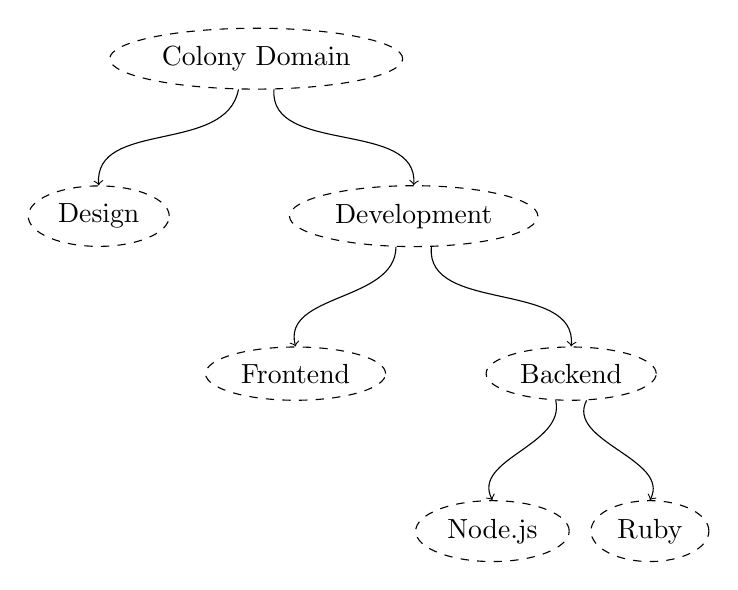
\begin{tikzpicture}
   \node[ellipse,draw, dashed] at (0,0) (tld) {Colony Domain};
   \node[ellipse,draw, dashed] at (-2,-2) (design) {Design};
   \node[ellipse,draw, dashed] at (2,-2) (development) {Development};
   \node[ellipse,draw, dashed] at (0.5,-4) (frontend) {Frontend};
   \node[ellipse,draw, dashed] at (4,-4) (backend) {Backend};
   \node[ellipse,draw, dashed] at (3,-6) (nodejs) {Node.js};
   \node[ellipse,draw, dashed] at (5,-6) (ruby) {Ruby}
    (tld.-120) edge[->, bend left=45, in=-120] (design.north)
    (tld.-60) edge[->, bend left=45, out=-60, in=120] (development.north)
    (development.-120) edge[->, bend left=45, in=-120] (frontend.north)
    (development.-60)  edge[->, bend left=45, out=-60, in=120] (backend.north)
    (backend.-120) edge[->, bend left=45, in=-120] (nodejs.north)
    (backend.-60)  edge[->, bend left=45, out=-60, in=120] (ruby.north);
 \end{tikzpicture}
 \caption{Parts of a possible domain hierarchy for a colony developing a web service.}
 \label{fig:domainhierarchysample}

\end{figure}

This compartmentalisation of activity in a colony provides a tangible benefit to the colony as a whole. When objections are raised, they can be raised to a specific level in the structural hierarchy provided by domains within a colony. This means that people with relevant contextual knowledge can be targeted for their opinion, and also means that when a dispute occurs the whole colony does not have to vote in the dispute. Only those users with the relevant skills are asked for their opinion.

We also note that on some level, it is up to individual colonies to decide how they wish to use domains --- some might only use them for coarse categorisations, whereas others may use them to very precisely group only the most similar tasks together, or even multiple tasks that other colonies would consider a single task. We aim to provide a general framework that colonies can use how they see fit, and to only be prescriptive in the service's use where necessary.

\newpage
\section{The Colonies' own Tokens}\label{sec:colony-tokens}
Every colony has its own tokens. These are the tokens that, when attached to a task bounty, confer reputation to the receiver. Beyond this, the tokens may be used in any number of ways; they may have financial value, or they may be purely symbolic (Section \ref{sec:colony-token-examples} below). The management of tokens falls to the token holders (Section \ref{sec:colony-token-management}).


\subsection{Managing a colony's token supply}\label{sec:colony-token-management}
A colony is in complete control of its own tokens. Crucially it is up to current token holders to decide on questions of token generation and destruction, and not up to reputation holders (alone).

\subsubsection{Initial Supply}
When a colony is created, the \ascode{TotalTokenSupply} and the \ascode{TokenIssaunceRate} are set. The former is the total number of colony tokens that will be created and the latter is the rate at which they become available to the colony-wide domain. Just as with any funding proposal (Section \ref{sec:finance}), users can issue a `ping' to update the totals available to the domain.

\subsubsection{Increasing the Token Supply}
To generate new tokens, there must be a large majority of current token holders in favour. Especially if the tokens have a financial value, it is crucial that new tokens cannot be generated without widespread consensus. Such decisions should therefore presumably have to be be made by a token-weighted vote with high quorum and majority requirements or possibly even a hybrid vote. How the latter option might work is described below:\\

In order to increase the \ascode{TotalTokenSupply} and thereby allow for new tokens to be generated, the following events must occur
\begin{itemize}
 \item A proposal is made to increase the value of \ascode{TotalTokenSupply}
 \item The proposal is backed by 10\% of all colony reputation
 \item A colony wide vote of tokens and reputation is held
 \item A majority of reputation voted in favour of the increase
 \item A two-thirds supermajority of tokens voted in favour
 \item Over 30\% of tokens participated in the vote.
\end{itemize}

\subsubsection{Changing the TokenIssaunceRate}
The \ascode{TotalTokenSupply} represents the tokens that the token holders have granted to the reputation holders in order to conduct business: to fund tasks and domains, to hire workers and contributors; especially during the early life of a colony in which it has litte to no revenue in other tokens to fall back on.\\
The \ascode{TokenIssaunceRate} is a measure of how rapidly the colony is able to absorb and allocate the new tokens. If the rate is `too high', tokens will accumulate in the colony wide domain's pot (or other pots lower in the hierarchy); usually this is not a big problem. If the rate is too low however, this signals that the colony has a healthy amount of activity and that the issuance rate has become a bottleneck. In such situations it may be desirable to increase the rate of issuance without necessarily increasing the maximum supply. \\
Increasing and decreasing the \ascode{TokenIssaunceRate} by up to 10\% can be done by the reputation holders alone and this action can be taken no more than once every 4 weeks. Bigger changes to the issuance rate require a double majority of tokens and reputation.


\subsection{Example of Token Usage}\label{sec:colony-token-examples}
\subsubsection*{Tokens as early rewards}
One of the chief benefits of having its own token is that a colony can offer rewards for work before it has any revenue or external funding to draw on. Similar perhaps to how a start-up company may promise stock options, a new colony may offer token bounties for tasks that people may accept in the hope that the reputation conferred by these token payments and the future revenue earned by the colony will eventually reap financial rewards. In other words it allows for `spending' before fund-raising and thus eases the start-up phase of new colonies. Later in its life, when the colony is profitable, payment in tokens could very well be the exception instead of the norm.
\subsubsection*{Tokens representing hours worked}
We could imagine a colony in which all tasks are paid in Ether or some other valuable token, but include a number of the colony's own tokens as well, equal to the expected number of \emph{hours worked} on a task. The members of the colony would be responsible for assigning `correct' token and Ether bounties to tasks; this extra cognitive workload would have the great benefit of solving the `Palo Alto Problem', in which users who are paid more for the same work - such as those living in Palo Alto may be compared to those in South America - earn more influence in the colony. 
\subsubsection*{Tokens as `upvotes'}
Tokens themselves need not have a monetary value; (a Colony could even chose (Section \ref{sec:colony-token-management}) to continually generate new tokens at an ever increasing rate to \emph{ensure} that they do not have a direct value). In such a situation, the token would only be valuable in a context in which payout also confers \emph{reputation}.
\newpage
\section{Reputation}
\subsection{What is Reputation?}
blabla text here ... score associated to an account... cannot be transferred... used as voting weight... hoepfully leading to meritocratic decision making.
FIXME FIXME

There are many reputation scores per user ... local to domains or skills.... not one global score. Also Reputation decays with time.



Reputation earned in Colony will primarily be earned from completing tasks, and the amount of reputation earned will be based on a combination of the performance of the user completing the task, and the payout associated with the task itself.

We note this creates a problem we have affectionately taken to calling the ‘Palo Alto Problem’, whereby users who are paid more for the same work - such as those living in Palo Alto may be compared to those in South America - earn more influence in the colony. While we would like to solve this problem, we have been unable to do so to date; any possible solution either seems to introduce a great deal of complexity to the system or provide the ability for a bad actor to accrue undue influence in the colony.
\subsubsection{Reputation per Domain}
Users have reputation local to any domain. Earning rep in a domain earns you rep in any parent domain. Losing rep also affects all children.
Top Level reputation ...

beyond this we also want skill tags:

\subsubsection{Skill hierarchy}

The existence of domains that form the organisational hierarchy of a colony was described in section \ref{sec:domains}. In addition to this organisational hierarchy (which is unique to each colony), the Colony Network also maintains a hierarchy of skill domains (or just `skills'), which is available for all colonies to use. A user's good or bad activity associated with either of these hierarchies will earn or lose them the corresponding reputation, though only in a single colony.\footnote{It is hopefully clear that allowing users to earn reputation in one colony and then use it to influence decisions in another would be ripe for abuse.}

For example, when a task is created, as well as being placed in a particular domain in the colony, it is also tagged with a skill from the skill hierarchy. When the worker earns reputation for succesfully completing the task, they will earn reputation in all the relevant domains and skills. Conversely, if they are to lose reputation because their work is found inadequate, they will do so in all the relevant domains ad skills.

\subsection{Earning reputation}
The only way that reputation is created in a colony is when it is FIXME

\subsubsection{Bootstrapping reputation}

Since a large portion of a colony's decision making procedure rests on reputation weighted voting, we are presented with a bootstrapping problem for new colonies.
When a colony is new, no-one has yet completed any work in it and so nobody will have earned any reputation. Consequently,no dospites could be resolved as no-one would be able to vote on them. \\
Therefore, when a colony is created, the creator can nominate addresses to have initial reputation assigned to them to allow the colony to bootstrap itself. There will be a global limit on the reputation that can be assigned in this manner in order to prevent an extreme reputation aristocracy. Given that reputation decays over time, this initial bootstrapping of reputation will not have an impact on the long-term operation of the colony. \textbf{This is the only time that reputation can be created without associated work being done.}

At first glance it may appear as if the same bootstrapping problem presents itself whenever a domain is created - if the domain has had no work done in it, then who has the authority to make decisions? We do not wish to allow the creation new reputation here, as this would devalue reputation already earned in the colony by users completing work. Luckily we can proceed without any new reputation: we simply accept the fact the new domain has no reputation in it. The colony is still able to make decisions and resolve disputes, because any objections can be escalated to a parent domain if necessary. Furthermore, even this escalation is not necessarily required in the event of a disagreement, because, even if there is no reputation in the domain to contribute to the decision, users will still be able to vote based on their reputation in relevant skills.

\subsubsection{Earning Reputation by contributing to a task}
admin, worker, evaluator.... FIXME

\subsubsection{Earning Reputation as a result of Disputes}
see title.



\subsection{Losing Reputation}

\subsubsection{Reputation Decay}
All reputation decays over time.\\
Every 600000 blocks, a user’s reputation in any domain or skill decays by a factor of 2. This decay occurs continuously, rather than being a step change every three months to ensure there are as few incentives to earn reputation at any particular time.

\subsubsection{Losing Reputation due to a Negative Evaluation}
working on a task. bad review. lose rep....


\subsubsection{Losing Reputation due to Bad Behaviour}
disputes and how they affect rep....


Whenever a user stakes tokens, they are also risking their reputation. If the tokens are lost, then they also lose reputation. Reputation is not staked, and so while at risk it can still be used by users to vote on decisions where that reputation is relevant - they only lose the voting power associated with the reputation once it is lost. However, it should be noted that the same is not true of colony tokens - once staked, their voting power is lost. However, we expect that users will only ever stake a small proportion of their tokens - only small amounts of tokens are staked in the Colony Network to ensure a tangible financial punishment to the staking user can be made if they are a badly behaving actor.

The amount of tokens to be staked and reputation that can be lost depend on the context of the action being taken. The greater the proportion of reputation in the colony that is potentially inconvenienced by the action being taken in the event that it is fraudulent, the greater the reputation and tokens that must be staked by the user to take the action.





\newpage

\section{Calculating Reputation: Miners and Merkle Proofs}\label{sec:reputationmining}
We see that the reputation system is a core component of any decentralised colony. By carefully balancing the rewards and penalties we aim to keep every users' incentives aligned with the colony and the colony network. Since reputation can only be \emph{earned} and not bought, the system fosters a more meritocratic from of decision making than pure token-weighted voting can hope to achieve. The continuous decay of reputation ensures that the influence conveyed by reputation is recent and up-to-date; it prevents a reputation aristocracy and allows for a fluid passing of control from one set of contributors to another over time.

How well the parameters of the reputation system balance out competing interests will have to be subject to empirical review when the colony network begins live operation and any parameters proposed in this document should be seen as suggestions, not prescriptions for the final network.

Due to the combined complexity of reputation scores across multiple colonies, domains and skills %; growing due to tasks completed and disputes won; shrinking due to decay and poor performance;
\textbf{reputation scores cannot be stored and calculated on-chain}. Instead, the calculations will all take place off-chain, the results of which will be reported to the blockchain by participating CLNY holders --- in a process resembling a proof-of-stake blockchain consensus protocol. We call this procedure \textbf{`Reputation Mining'}.\\
The reputation calculation whose result the miners are submitting, is determined by the activities that have taken place in the colonies and can be fully deterministically derived from the ethereum blockchain. Game-theoretically the system is protected similarly to the off-chain calculations of truebit (\cite{TruebitWhitepaper}) in that, \emph{while the calculation cannot be done on-chain and a correct submission can never be proved true, an incorrect calculation can always be proved to be wrong.}


\subsection{The Reputation Tree and the ReputationRootHash}\label{sec:reptree}
A reputation consists of the following data:
$$
R = 
\begin{cases}
 rep\_id & \textnormal{the id of a skill or domain identifying the type of reputation},\\
 colony\_id & \textnormal{the colony the reputation is held in},\\
 user & \textnormal{the address holding the skill},\\
 amount & \textnormal{the numerical value of the reputation}.
\end{cases}
$$
All individual reputations are assembled into the \textbf{``Reputation Tree''} which is a merkle tree (\cite{MerkleTrees}, \cite{MerkleInEthereum}) of all individual reputations in a colony and the cumulative totals. (Note: The tree also contains the totals of all types of reputation held by users in this colony; these are entries in which the \ascode{user} is set to zero.)\\
All reputations held by all users in all colonies are ordered in a list. The elements of this list are hashed pairwise, to end up with a shorter list of hashes. This process is repeated until only one hash remains: the \ascode{ReputationRootHash}, $\mathcal{RH}$.
\begin{center}
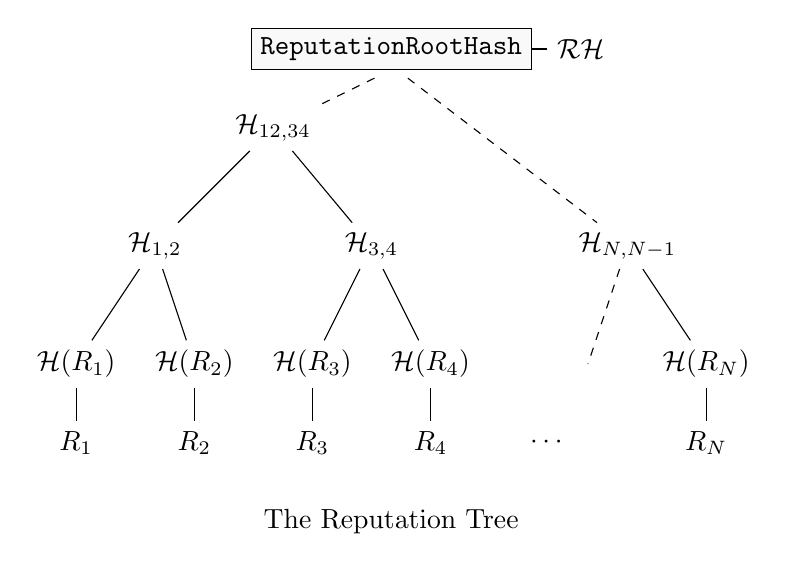
\begin{tikzpicture}
 \node at (0,-5) (r1) {$R_1$};
 \node at (1.5,-5) (r2) {$R_2$};
 \node at (3,-5) (r3) {$R_3$};
 \node at (4.5,-5) (r4) {$R_4$};
 \node at (6,-5) (rdots) {$\cdots$};
 \node at (8,-5) (rn) {$R_N$};
 %
 \node at (0,-4) (r1hash) {$\mathcal{H}(R_1)$}
  edge[-] (r1);
 \node at (1.5,-4) (r2hash) {$\mathcal{H}(R_2)$}
  edge[-] (r2);
 \node at (3,-4) (r3hash) {$\mathcal{H}(R_3)$}
  edge[-] (r3);
 \node at (4.5,-4) (r4hash) {$\mathcal{H}(R_4)$}
  edge[-] (r4);
 \node at (8,-4) (rnhash) {$\mathcal{H}(R_N)$}
  edge[-] (rn);
 %
 \node at (1,-2.5) (r12) {$\mathcal{H}_{1,2}$}
  edge[-] (r1hash)
  edge[-] (r2hash);
 \node at (3.75,-2.5) (r34) {$\mathcal{H}_{3,4}$}
  edge[-] (r3hash)
  edge[-] (r4hash);  
 \node at (7,-2.5) (rnn) {$\mathcal{H}_{N,N-1}$}
  edge[-] (rnhash)
  edge[dashed] (6.5,-4);
 %
 \node at (2.5,-1) (r14) {$\mathcal{H}_{12,34}$}
  edge[-] (r12)
  edge[-] (r34);
 %
 \node[draw, fill=gray!5] at (4,0) (root) {\texttt{ReputationRootHash}};
 \node[right = 2mm of root] (rh) {$\mathcal{RH}$} 
   edge[-] (root);
 \node[below = 1mm of root] (dummy) {\phantom{a}}
  (dummy.north west) edge[dashed] (r14)
  (dummy.north east) edge[dashed] (rnn);
 %
 %
 \node at (4,-6) (label) {\textnormal{The Reputation Tree}};
\end{tikzpicture}
\end{center}

In the event of a starting or an intermediate array being an odd number (which will always happen for a starting array that is not a power of two), the hash contained in the last element is hashed with itself.

The \ascode{ReputationRootHash} is the data we record on the blockchain. It represents an integrity check for the entire reputation system and whenever a user wishes to make use of their reputation, the can submit a merkle proof starting at the reputation $\mathcal{R}_i$ they wish to make use of and ending at $\mathcal{RH}$.

\subsection{Calculating the new root hash}
To calculate the new root hash, the miners begin with the last reputation state, and decays all reputations held by all users in all colonies, in the order of the leaves in the tree. They then take the set of reputation gains or losses due to good or bad behaviour that were not in the last state submitted, and are to be included in the next state. They apply the reputation updates to each user, in each colony, to end up with a new list of reputations for all users and colonies. These new reputations are then hashed and assembled into a new merkle tree yielding an updated \ascode{ReputationRootHash}.

While the calculation is too large to be done on-chain due to technical (gas limit) and economic (gas cost) limitations, it is expected that this calculation can easily be performed by any consumer grade laptop computer.

\subsection{Submission of a new root hash}
%
\subsubsection*{What is submitted?}
The final \ascode{ReputationRootHash} is submitted to the contract by the miner along with the number of leaves in the tree. Further, the miner also submits the IPFS/Swarm hash of a document containing the entire state tree (though this is only for convenience; any user can construct this locally based on the blockchain history).
%
\subsubsection*{Who can submit a new root hash?}
CLNY token holders are eligible to become miners and participate in the reputation update process, but since any user can calculate the correct root hash locally, it would be possible for \emph{any} \rcth\ to submit the hash to the contract.
It is however undesirable to have too many submissions for every update. We propose a mechanism that only allows some miners to submit results to begin with. To participate in the mining process, \rcths\ must stake some of their tokens to become `reputation miners'. A submission will only be accepted from a miner if \ascode{SHA3(address, N, hash)} is sufficiently small (\ascode{< target}). At the beginning of the submission window, the target is set to 0 and slowly increases to $2^{256}\times10^{-3}$ after 150 blocks. The fact that the target is capped, rather than increasing to $2^{256}$ at the end of the submission period effectively creates a minimum number of tokens required to submit a hash. This puts a tangible cost on any attacks revolving around spamming known false submissions (see section \ref{sec:mining-possible-attacks}). This factor will be changeable by the \rc.

The variable $N$ that goes into the hash is some number greater than 0 and less than the number of tokens the \rcth\ address has staked divided by $10^{15}$, meaning that users with a large stake have a higher chance of qualifying to submit a hash than smaller stake holders. The factor of $10^{15}$ is introduced to ensure that all hashes a user is eligible to submit can be calculated in a few seconds by the client.
%
\subsubsection*{Verifying a submission}
If only one state is submitted by the end of the submission period, then the new state is accepted, and proposals of the next state can begin to be made. This is expected to be the most common occurrence.\\
If more than one state has been submitted, then either someone has made a mistake, or there is a malicious entity trying to introduce a fraudulent reputation change. In this event, the a challenge-response protocol can establish which state is incorrect (see Section \ref{sec:challengeresponse})

\subsubsection*{Mining Rewards}

When a state is accepted, a small number of (newly generated) \rcts\ are made available for the user who first submitted the correct state to claim as a reward. When the user claims this payout, they receive a corresponding amount of reputation in the \rc\ (a special mining skill, which only users in the root colony can earn by performing this task). This reputation update is no different from any other, aside from the limitations of who is able to earn it, and will be included in a subsequent reputation update cycle.

\subsection{Dealing with false submissions}\label{sec:challengeresponse}
The challenge-response mechanism detailed below relies heavily on merkle proofs, so it will be useful to establish some notation.

\subsubsection{Merkle Proofs}
Consider the merkle tree shown in figure below. In order to prove that the element \ascode{A} is in the tree with root \ascode{G}, one submits a merkle proof containing the following information: \ascode{A, [B,F], [l,l]}. The first argument is the element whose existence is to be proved. The second argument is the list of hashes that \ascode{A} should be hashed pairwise with. The last argument is an array of \ascode{l}'s and \ascode{r}'s that indicates whether the hash calculated so far should be hashed on the left or the right of next element in question. So to show that \ascode{C} was in the tree with root \ascode{G}, the proof would be of the form \ascode{C, [D,E], [l,r]}.
\begin{center}
 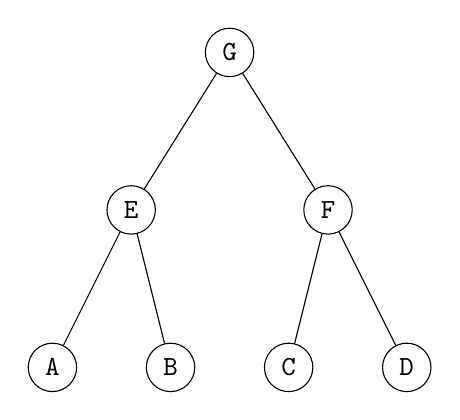
\begin{tikzpicture}
  \node[shape=circle, draw] at (0,-4) (a) {\texttt{A}};
  \node[shape=circle, draw] at (1.5,-4) (b) {\texttt{B}};
  \node[shape=circle, draw] at (3,-4) (c) {\texttt{C}};
  \node[shape=circle, draw] at (4.5,-4) (d) {\texttt{D}};
  %
  \node[shape=circle, draw] at (1,-2) (e) {\texttt{E}}
   edge[-] (a)
   edge[-] (b);
  \node[shape=circle, draw] at (3.5,-2) (f) {\texttt{F}}
   edge[-] (c)
   edge[-] (d);
  %
  \node[shape=circle, draw] at (2.25,0) (g) {\texttt{G}}
   edge[-] (e)
   edge[-] (f);
 \end{tikzpicture}
\end{center}
Note also that the array of \ascode{l}'s and \ascode{r}'s nothing more than a binary representation of the leaf node's index in the tree. When expressed in this way, we refer to the index as the `path' in the merkle proof. We refer to the objects that get hashed along the way (e.g. \ascode{[D,E]}) as the `siblings'.
%
\subsubsection{The Challenge-Response Protocol}
We assume that the correct hash is one of the  submitted hashes. This is a reasonable assumption, as only one out of all the miners is required to make a correct submission, and there is an incentive for them to do so (Section \ref{subsec:mining-costs-and-rewards}). Thus our task is not to validate the correct hash but to invalidate the false ones.

We must prove all but one submission incorrect by having each submission navigate a series of challenges. These \emph{challenges} refer to events that happened in the colony network within the last update cycle that have a reputation effect while the \emph{responses} to the challenges are merkle proofs that the corresponding reputation update was properly handled.

\subsubsection*{1. The Justification Tree}
 The first step is for both parties to upload a second merkle root. This is the root of a tree where each leaf represents a complete reputation state i.e. each leaf is a \ascode{ReputationRootHash}. The right-most leaf ($\mathcal{RH}_n$) is the hash they originally submitted, the left-most leaf ($\mathcal{RH}_0$) is the final accepted reputation state from the last update, and the intermediate leaves ($\mathcal{RH}_i$) represent the evolution of the reputation state after the reputation updates are applied one-at-a-time. 
 %
 \newcommand{\jrh}{\ensuremath{\mathbb{JRH}}}
 %
\begin{center}
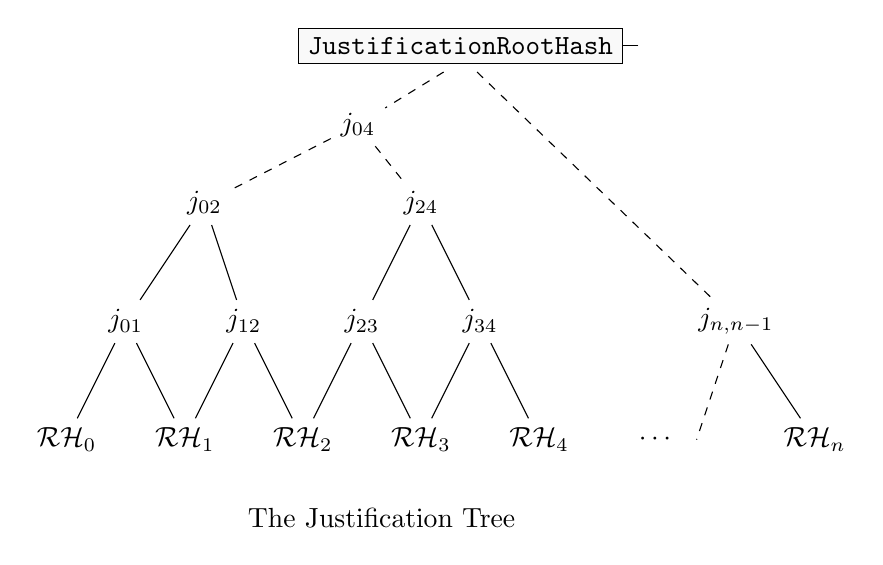
\begin{tikzpicture}
 \node at (0,-4) (rh0) {$\mathcal{RH}_0$};
 \node at (1.5,-4) (rh1) {$\mathcal{RH}_1$};
 \node at (3,-4) (rh2) {$\mathcal{RH}_2$};
 \node at (4.5,-4) (rh3) {$\mathcal{RH}_3$};
 \node at (6,-4) (rh4) {$\mathcal{RH}_4$};
 \node at (7.5,-4) (rdots) {$\cdots$};
 \node at (9.5,-4) (rhn) {$\mathcal{RH}_n$};
 %
 \node at (0.75,-2.5) (rh01) {$j_{01}$}
  edge[-] (rh0)
  edge[-] (rh1);
 %
 \node at (2.25,-2.5) (rh12) {$j_{12}$}
  edge[-] (rh1)
  edge[-] (rh2);
 %
 \node at (3.75,-2.5) (rh23) {$j_{23}$}
  edge[-] (rh2)
  edge[-] (rh3);  
 %
 \node at (5.25,-2.5) (rh34) {$j_{34}$}
  edge[-] (rh3)
  edge[-] (rh4);  
 %
 \node at (8.5,-2.5) (rhnn) {$j_{n,n-1}$}
  edge[-] (rhn)
  edge[dashed] (8,-4);
 %
 \node at (1.75,-1) (rh02) {$j_{02}$}
  edge[-] (rh01)
  edge[-] (rh12);
 %
 \node at (4.5,-1) (rh24) {$j_{24}$}
  edge[-] (rh23)
  edge[-] (rh34);
 %
 \node at (3.7,0) (dummy14) {$j_{04}$}
  edge[dashed] (rh02)
  edge[dashed] (rh24);
 %
 \node[draw, fill=gray!5] at (5,1) (root) {\texttt{JustificationRootHash}};
 \node[right = 2mm of root] (jrh) {$\jrh$} 
   edge[-] (root);
 \node[below = 1mm of root] (dummy) {\phantom{a}}
  (dummy.north west) edge[dashed] (dummy14)
  (dummy.north east) edge[dashed] (rhnn);
 %
 %
 \node at (4,-5) (label) {\textnormal{The Justification Tree}};
\end{tikzpicture}
\end{center}
Note that in the first stage of the tree, every neighbouring pair of leaves is hashed, and so any pair has a shared merkle proof to the root.\\
Any two differing submitted states agree on the first leaf $\mathcal{RH}_0$ (the \ascode{ReputationRootHash} accepted at the end of the previous iteration of the mining process), and disagree on the last leaf $\mathcal{RH}_n$. Somewhere there is a transition  ($\mathcal{RH}_i$ to $\mathcal{RH}_{i+1}$) where they agree on the starting state but disagree on the result. This transition is meant to be the effect of a single reputation update, the calculation of which is able to be done on-chain. \\
First, however, we must establish where the two overall calculations submitted differ.

\subsubsection*{2. Searching for the discrepancy}
The contract requires both parties to submit merkle proofs that specific reputation updates were handled correctly. It begins by pseudorandomly picking a reputation updating transaction from the first half of the log (Appendix \ref{appendix:rep-transfer}) (say the $i^{th}$ update for some $i<\frac{n}{2}$) and requires both parties to provide:\\
\begin{itemize}
 \item[(i)] The root hash before the update was applied ($\mathcal{RH}_{i-1}$)
 \item[(ii)] The root hash after the update was applied ($\mathcal{RH}_i$)
 \item[(iii)] A merkle proof showing that the pair ($\mathcal{RH}_{i-1}, \mathcal{RH}_i$) is correctly included in the justification tree
\end{itemize}

The contract then repeats this process using a binary search algorithm. If the merkle proof (iii) for both submissions had the same sibling values almost all the way up, but differing only in the the final sibling, then the discrepancy must occur later (i.e. the two sumbissions differ at some $i^\prime > \frac{n}{2}$) whereas if the merkle proofs already differ at an earlier sibling, then the submissions must also differ in an update before $\frac{n}{2}$. This final hash is stored as the new target hash for following challenges.

The contract pseudorandomly selects a reputation update from within the subtree in which the first discrepancy is known to lie. Each newly submitted proof further reduces the size of the subtree by a factor of two\footnote{By examining precisely at which sibling the first discrepancy occurs, some stages of the binary search could be skipped. However, in order to accomplish this all the siblings of the proof that first completed the challenge would need to be stored on the blockchain, so it’s likely that it is more gas efficient to just do the `na\"{i}ve' binary search.}.

If at any point in the process, a submission does not respond to the challenge, in a timely fashion they forfeit, and are assumed to be incorrect. If all submissions continue to be defended successfully, ultimately, the location of the first discrepancy in the series of state transitions is found: the submissions agree on (i) but not (ii). The contract then requires
\begin{itemize}
 \item[(iv)] A merkle proof for the reputation ($R_j$) affected by the $i^{th}$ update transaction.
\end{itemize}
Note: in point (iv), the \emph{exact same} merkle proof that proves the inclusion of $R_j$ (before the reputation update) in the root $\mathcal{RH}_{i-1}$ must also prove the inclusion of $R_j$ (after the reputation update) in the root $\mathcal{RH}_i$. This is because the trees $\mathcal{RH}_{i-1}$ and $\mathcal{RH}_i$ differ in only a single leaf.\\

Finally, this transition is then calculated on-chain to determine which is the correct answer. The submission that has been proved to be incorrect is rejected.

In the event of more than two submissions, this process is conducted in parallel between multiple pairs of submitted hashes, and then repeated, until only one submission remains.

If less than an hour elapses from submissions opening to only one submission remaining, the next submission window only opens when a hour has passed from the start of this window. If more than an hour has passed, the next submission window opens immediately.



\subsection{Implementation Details}\label{sec:mining-implementation-details}
%
\subsubsection{Keeping track of reputation changes}
%
There are two types of reputation update that occur:
\begin{itemize}
 \item Decay of existing reputation
 \item Addition or removal of reputation as a reward or punishment.
\end{itemize}
All reputation decays, and so it is only the latter that is explicitly recorded on the blockchain when an event occurs. Specifically, when a reputation affecting event occurs, an entry is added to the `reputation update log' in the \rc. Such an entry consists of
\begin{center}
\begin{tabular}{lll}
$R$ &--& The reputation to be updated\\
$\Delta_R$ &--& The reputation change\\
source &--& An address if the reputation is coming from someone, zero otherwise\\
$n\_updates$ &--& The cumulative number of all reputation changes that will have been made\\
	    & & when this log entry is correctly processed.\\
\end{tabular}
\end{center}

Recall also from section \ref{sec:reptree} that a reputation consists of
\begin{center}
\[
R = 
\begin{cases}
 rep\_id & \textnormal{the id of a skill or domain identifying the type of reputation},\\
 colony\_id & \textnormal{the colony the reputation is held in},\\
 user & \textnormal{the address holding the skill},\\
 amount & \textnormal{the numerical value of the reputation}.
\end{cases}
\]
\end{center}

%I suggest we do a little appendix of data structures. That way we can refer to reputations and rep_ids an other data here without having to fully document it here. We would not need to even mention the parent_id and parent_n_id here (as we need it onle elsewhere)...

Furthermore for each $rep\_id$, the following data is also known
\[
  rep\_id \rightarrow 
  \begin{cases}
    parent\_id &	\textnormal{the rep\_id of the parent domain/skill}\\
    parent\_n\_id &	\textnormal{the rep\_id of the $n^{th}$ parent}\\
    generation &	\textnormal{total number of parents}\\
    children\left[\cdots\right] &	\textnormal{array of children}\\
    n\_children &	\textnormal{total number of children}
  \end{cases}
\]
When a user earns reputation in a skill or domain, s/he also earns reputation in all parents and thus corresponds to \ascode{generation+1} number of reputation updates. Alternately, when a user loses reputation, they also lose reputation in all parents and all children representing a total number of updates of \ascode{generation + n\_children + 1}. (Note: parent\_id and parent\_n\_id are not used here; they are used during dispute escalation - see Section \ref{sec:disputes}).

It is only by recording the number of parent reputations (\ascode{generation}) and how many reputations have been updated already in this update cycle (via \ascode{n\_updates}) that the resolution protocol is able to perform the binary search of the justification state trees submitted by the disagreeing users. At the start of the challenge protocol, the contract can look up the last entry in the update table for the cycle under consideration, and work out how many updates have occurred in this cycle based on the number of updates prior and the number of parent reputations. It can then conduct the binary search.

When the discrepant state transition is found, the users supply the index of the update on-chain that corresponds to that reputation update. This means that the contract does not have to iterate over the whole list expensively, but the contract can easily check the correct reputation update is being considered, and then confirm that the calculation made corresponds to the correct reputation update. In the event that the discrepant transaction is a decay transaction, which is easily determined by the merkle path corresponding to an index smaller than the number of leaves in the tree at the end of the last successful update, they must also supply a merkle proof that the starting value assumed for the user corresponds to the value that user had at the end of the last update cycle.

Recording the number of leaves in the tree is required to allow the binary search to occur and accommodate the decay calculations that must be done at the start of each update. Before any new reputation is earned or lost in an update cycle, all existing reputations owned by users decays (see next section \ref{sec:repdecay}). There is a decay calculation for every leaf in the previously accepted tree. We do the decay calculations first to give users the benefit of the doubt during reputation updates so they do not lose reputation they have only just earned to premature decay.

When a user earns reputation in a new skill, at least one new leaf is added to the tree - if they have not earned reputation before in some of the parents, then they will also cause further new leaves to be added. New leaves will also be added if they are the first user in a colony to earn those particular skills, making the total reputation for that skill in the colony non-zero. During a dispute, when the user proves that they have included the update in the tree, it is not possible to check (efficiently) on-chain that they should not have added it to an existing leaf instead. However, because during a dispute we are always playing two submissions off against the other, one of two things will be true:
\begin{itemize}
 \item Both submissions add a new leaf to the tree. If there was a discrepancy, then it is in the maths conducted on this leaf, not the addition of the leaf itself. The maths can be checked on-chain to establish which result is correct.
 \item The other submission adds the new reputation to an existing leaf (the correctness of which can be checked on-chain easily). In this case, the user who added the leaf incorrectly is wrong.
\end{itemize}





\subsubsection{Transfers of reputation between accounts}\label{sec:reptransfer}

The most important quality of reputation that distinguishes it from a token is that it is tied to an account and cannot be transferred. However, in the event of disputes (Section \ref{sec:disputes}) it can happen that one party to a dispute loses reputation while the other gains. This process has to be modelled as a `reputation transfer' to ensure that reputation is never created in this process (i.e. the reputation lost by the loser is at least as much as the reputation gained by the winner).

If an entry in the reputation update log indicates that the reputation has come from another user, then this entry represents updates of all the parents of the reputation being gained by one user, and updates of all the parents and children of the reputation being lost by the other. However, we have to ensure that the user who is losing reputation still has the reputation to lose if another user is gaining it.

To achieve this, all the transactions that correspond to updating the reputations of the user gaining the reputation are done first. In the event such a transaction must be proved to be correct in the resolution protocol, the users can provide a proof of the losing user’s reputation, prior to them losing it in this update, and this can be compared to the amount of reputation intended to be gained. Whichever is smaller is used as the amount of reputation the user is gaining during the calculations.

Then, when calculating the reputation deduction to be applied to the losing user, the reputation that was used for as the voting weight should be done last i.e. all the children (and parents) should be considered first, as it is the amount of the reputation that was eligible to vote that will determine the fraction lost of each of the children reputation. %If any of these calculations need to be proved correct during the resolution protocol, 

For further details about reputation transfers and disputes, see Appendix \ref{appendix:rep-transfer}.

\subsubsection{The Reputation Decay Process}\label{sec:repdecay}
The reputation decay process was describe above as being continuous. To have a user's reputation continuously decay, and end up with half of the starting amount after three months, an exponential decay makes most sense. However, such a calculation is not possible on-chain, so we must use an approximation. The details of the approximation we use, and a proof that this approximation is accurate and will not affect the running of (active) colonies can be found in appendix \ref{appendix:rep-decay}.


\subsection{Possible Attacks}\label{sec:mining-possible-attacks}
\subsubsection*{Many false submissions and Denial of Service}

In the event of multiple submissions, finding the correct one takes time --- the timeout $t$ for the challenge-response must be reasonable to allow the transaction defending a submission to propagate and be mined. A denial-of-service attack is therefore possible, whereby an attacker makes many false submissions. However, if these false submissions were random hashes, unable to be defended, then none would be defended correctly within the first five minute window, and the attack would quickly end. 

The denial of service attack (the delay of a proper reputation update) can only be sustained when the false submissions are incorrect only in some leaves, and the majority of the state tree is correct. In this scenario, the attacker successfully defends each of their submissions for as long as possible to delay the resolution of the reputation mining protocol as much as possible.

Any such attack is capped by the first round of pairings of submissions against each other. Even if the attacker made millions of submissions, only a finite number of those would be able to be successfully defended due to the block size --- currently, no more than 4500 submissions would be able to be defended, even if the attacker used up all block space during the timeout.\footnote{These figures assume $1.5\pi\times10^6$ gas in a block, and that each transaction is only 21000 gas for a worst-case-scenario calculation.} With only 4500 submissions able to make it to the second round, the length of time the DoS attack would be sustained for is given by 

$$t \times \left\lceil\log_2\left(4500\right)\right\rceil\times \left\lceil\log_2\left(N_{\rm updates}\right)\right\rceil$$

\noindent where $N_{\rm updates}$ is the number of reputation updates that have been made in this update cycle. To arrive at this figure, we know there will need to be $\left\lceil\log_2\left(4500\right)\right\rceil$ rounds of comparison between submissions to eliminate all but one. Each round will require $\left\lceil\log_2\left(N_{\rm updates}\right)\right\rceil$ interrogations of the justification tree to establish where the two submissions being compared differ. Finally, each interrogation can take up to $t$ before it is considered to have timed out and one or both of the submissions is deemed invalid. The product of these three factors tells us how long this reputation update can be delayed by an attacker.

Long term, $N_{\rm updates}$ will be dominated by the decay transactions rather than by any updates that have occurred since the last reputation state was established. Even if the Colony Network were wildly successful, with 100000 colonies, each with 1000 users that had earned some reputation in 1000 different skills in each of the structural and skill hierarchies, the delay to the reputation updates would only be around $36$ hours.

There would be little effect on the rest of the colony network in this time. Users would still be able to exercise their reputation from the previous reputation update, and continue to influence decisions with that reputation. Indeed, this shows what perhaps the main motivation for such an attack would be --- if a user knew that they had been `caught' behaving badly, and was due to lose all their reputation, they might try such an attack to eke out the last bits of influence they possibly could. However, decisions in the colony network do not resolve quickly, and in a well-developed colony we would not expect any one person to have a large amount of reputation when compared to the rest of the colony, so it seems unlikely they would be able to unduly influence decisions significantly while conducting the attack.

Assuming this attack continued, then the reputation mining protocol would effectively only update every 36 hours. Users staking would become more susceptible to variance in terms of the rewards, but otherwise little would change in the day-to-day functioning of any individual colony. 

However, the attacker would lose \emph{all} the \rct\ that they had staked (which would be around 4500 times the expected minimum stake) in order to perform the attack, and so would have to buy more to attack again making this attack exceedingly expensive.


Note: There is an edge case to consider in which the attacker is sending enough defending transactions to completely fill the blocks. In such a case however we assume that the defence of the legitimate state is always successfully included in block, as a one-off increase in gas costs will always be worthwhile to ensure the legitimate state is defended.  

\subsection{Costs and Rewards of Mining}\label{subsec:mining-costs-and-rewards}
In order to be involved in the reputation mining process, \rcths\ must stake their tokens with the Colony Network Contract. This allows them to submit a reputation hash as part of the reputation mining process described above.

If they submit a new hash, this is recorded and they are noted as the first address to submit that hash. If they submit a hash that has already been submitted, they are appended to a list of users that have submitted that hash.

If a hash is found to be incorrect, all those who submitted it lose their stake. If a hash is found to be correct, however, the users who submitted it gain root colony tokens and reputation. The total amount of reputation earned is controlled by the amount of reputation that exists in the colony, and tries to ensure that 25\% of the reputation in a colony comes from mining. If normal activity in a colony generates $A$ reputation per hour, the total reputation that exists $R$ is given by 

$$\frac{A}{1-\exp\left(-k\right)}$$

\noindent where $k$ is the decay constant used in each update period (see Appendix \ref{}). If we wish for 25\% of $R$ to come from mining, then the amount of reputation earned from mining in each update period should be 

$$\frac{R}{4}\left(1-\exp\left(-k\right)\right).$$

When a user makes their submission, their weighting for that hash is recorded, and the total weight submitted by all users for that hash is updated. A staker's weight is given by 

\begin{equation}\label{eq:stakerweight}
\left(1-\exp\left(-\frac{t}{T}\right)\right) \times \frac{1}{n+S} \times B
\end{equation}

where $B$ is the total number of tokens they have staked, $n$ is their position in the list, $S$ and $T$ are normalising constants, and $t$ is the number of blocks they have staked their tokens for. 

The first factor in equation \eqref{eq:stakerweight} encourages users to stake their tokens for long periods of time. After $T$ blocks, this first factor is 0.63 of what it will eventually grow to given unlimited time. We expect $T$ to represent around a month.

The second factor in equation \eqref{eq:stakerweight} encourages users to submit the hash as soon as possible, with this factor becoming smaller the later users submit; the first submission will have approximately twice the weight of the last submission, all other factors being equal. This factor also means that users are not incentivised to split up their holdings, as some of the split up tokens will have lower weightings. $S$ should be a number on the order of the number of people that are staking in each round to ensure the discrepancy between the rewards for being first and last are not huge; it should be under the control of the \rc.

The last factor $B$ is the number of tokens the user has staked --- if they have staked more tokens, they get more of the payout than they would have done if they had staked less.


%Notes:\\
%-token holders must stake in order to be miners\\
%-reputational reward comes from tokens earned just like task payout
%-how much rep exactly you get (similar to 5 star rating for work) determined by how long you lock your tokens. Short term = 3 stars, long term 5 stars.\\
%-how many tokens are paid out to miners must vary as the price of the token changes. Idea: make it scale with the total paid out in other domains of root colony. If feasible, use one month rolling average. Prevent miners overpowering rest of root colony with too much reputation.
%- $k$ should be multiplied by the number of hours since the last update to accommodate for attack
%- Merkle proof of current $R$ should be submitted with hash, otherwise not accessible on-chain?

\newpage


\section{Finance}\label{sec:finance}


%This is a work in progress. Aron is working on it.



\subsection{Tokens and Ether}
Every colony has its own ERC20-compatible token, the `local colony token'. These tokens are under the control of the colony contract and may be used to pay for work done in the colony. Tokens only leave the control of the colony upon being paid out for completed tasks.\\
In addition to local tokens, a colony may also use Ether, Global Colony Tokens and several other ERC20 tokens that have been explicitly whitelisted by the Colony Network.


\subsection{Pots and Funding Proposals}
All tokens and currencies are administered by the colony contract; it is responsible for all the bookkeeping and allocations.\\
\textbf{Each domain and each task in a colony has an associated \emph{pot}.} To each pot, the colony contract may associate any number of unassigned tokens it holds. Depending on context, the funds in a pot may be referred to as the bounty, the budget, the salary or woking capital.\\
\textbf{Funds are transferred between pots through \emph{funding proposals}.}
\begin{description}
 \item A Funding Proposal consists of the following data
 \begin{itemize}
  \item \textbf{Creator}	--	The person that created the proposal.
  \item \textbf{From}	--	Pot funds are coming from
  \item \textbf{To}	--	Pot funds are going to
  \item \textbf{TokenType}	--	The token contract address (0x0 for ether)
  \item \textbf{CurrentState}	--	The state of the proposal ( e.g. inactive, active, completed, cancelled )
  \item \textbf{TotalPaid}	--	How much has been transferred along this funding proposal so far
  \item \textbf{TotalRequested}	--	The maximum amount to transfer after which this funding porposal is considered 'completed'
  \item \textbf{LastUpdated}	--	The time when the funding proposal was last updated
  \item \textbf{Rate}	--	Rate of funding
 \end{itemize}

\end{description}
We distinguish between two types of funding proposals; one intended for normal use, and one intended to be used when atypical circumstances present themselves (a \emph{mandated funding proposal}). The funding proposal intended for normal use may start funding the target straight away, whereas a mandated funding proposal must be explicitly voted on before it starts directing funds. Furthermore, in a normal funding proposal the target pot must be a direct descendant of the source in the hierarchy whereas a mandated funding proposal has not such restrictions.\\
Mandated funding proposal should be used: when funds need to be directed somewhere that is not a direct descendant of the source or when the funding rate needs to be very high (fast/immediate payment), or when the funding rate should be otherwise controlled (eg. salary).\\

In either case, the assignment to pots associated with departments or tasks is purely a bookkeeping mechanism; from the perspective of the blockchain, ether and tokens are held by the colony contract until paid out when a task is completed. 

\subsubsection*{Creating a Funding Proposal}
Any member of the colony may create a funding proposal, however, the user in question must stake 0.01\%\footnote{this value may change before release} of the relevant reputation, where the reputation in question is that of the domain that is the most recent common ancestor of the source and target pots. They must also stake the same fraction of the colony's tokens i.e. the amount of reputation being staked is as a fraction of reputation in the whole colony domain, an the user must stake that fraction of all of the colony's local tokens in existence. This small stake is used to help discourage spamming of funding proposals and provide a mechanism whereby the creator can be punished for bad behaviour. 

\subsubsection*{From, To and TokenType}
The purpose of a funding proposal is to move tokens of \textbf{TokenType} from a pot \textbf{From} to a pot \textbf{To}. \\
The TokenType may be any ERC20 token whitelisted by the network, ether, Global Colony Token or Local Colony Token. The `From' and `To' addresses must be pots associated with a domain or a task in the colony. If the funds are to move `downstream' from a domain to one of its children, a regular funding proposal is often sufficient. To move funds between any other pots or at a higher priority / rate, a mandated funding proposal is needed.

\subsubsection*{CurrentState}
The state of a funding proposal is either `inactive', `active', `completed' or `cancelled'. Only an active funding proposal is in line to receive any funds. A regular funding proposal begins in active state while a mandated one begins inactive (i.e. it must be activated by a dispute / vote). A funding proposal is completed when it's `TotalPaid' reaches `TotalRequested'. Any other state changes must be made through the dispute mechanism.

\subsubsection*{TotalPaid and TotalRequested}
The total number of funds that a funding proposal wiches to reallocate is called its `TotalRequested' amount. Due to the mechanism by which funding proposals accrue funds over time, it is common that a funding proposal will have received a part but not all of its TotalRequested amount. The total number of tokens accrued to date are stored in its `TotalPaid' amount. 

\subsubsection*{Rate and LastUpdated}
When a funding proposal is elligible to accrue funds (see below QUEUE REFREFFERERENCE) it does so at a specific Rate. Since nothing happens on the blockchain without user interaction, the funding system uses a form of lazy evaluation. To claim funds that the proposal is due, a user may `ping' the proposal -- the user requests and update. Upon being pinged, the time since LastUpdated is multiplied by the Rate to determine how many tokens the proposal would have accrued in the interim if funding flow were continuous. This amount is added to TotalPaid and the current time is recorded as LastUpdated.\\
Note: TotalPaid in only ever increased up to TotalRequested and when this happens, the LastUpdated value is set to the earliest time at which this could have occured.

\subsubsection{The Funding Queue}
Active Funding Proposals that share the same `From' pot are ordered in a queue. At the top of the queue are the mandated funding proposals, followed by the regular funding proposals. MFPs are ordered by the total reputation in their domain\footnote{The domain of an MFP is the domain that voted on it becoming active - usually this is the last common ancestor of the source and target pot domains.} - while regular funding proposals are ordered by `backing'.  The details of this procedure are outlined below REFREFFERERENCE.\\



Insert schematic picture here of funding proposals in a queue.\\[2cm]








\subsubsection{Regular Funding Proposals}
A regular funding proposal (\textbf{RFP}) is a funding proposal from some domain's pot to one of it's children's. It starts out in the active state and is thus immediately elligible for funding. It may be cancelled at any time by the creator, or through the dispute mechanism.

\subsubsection*{Ordering of RFPs}
Regular funding proposals are ordered in the \emph{Funding Queue}. Only one of them can receive funds at any one time. The proposals are ordered by `amount of reputation backing the proposal'.\\
When created, a regular funding proposal gets placed at the bottom of the queue. Users can give a proposal `backing' weighted by their reputation in the source domain\footnote{The source domain of an RFP is the domain of the pot that the funding proposal is `From'.} at the time of backing\footnote{A user's reputation may change, but the backing weight is recorded at the time of backing and does not change without further user action.}. There are no costs to backing a proposal (other than gas costs) and the users obtain no direct benefits; it does not represent them `staking their reputation', it merely helps the proposal achieve funding.

The more reputation backs a proposal, the higher up the queue it is placed. Every transaction that adds backing to a proposal (or otherwise updates the backing level) inserts the proposal in the correct place in the queue. Only the funding proposal at the top of the queue accrues funds.\\

\subsubsection*{The Rate of funding for RFPs}
The more reputation backs a proposal, the faster it is funded; the rate scales linearly, and at the limit, if 100\% of the reputation in the source domain backs a regular funding proposal, then that funding proposal will be funded at a rate of 10\%\footnote{This number may change before release} of the domain's holdings (of the TokenType) per day. This ensures that, in the event of the queue being empty, the opportunistic user is unable to claim the entirety of the domain's funds instantaneously.

When a user backs a proposal, both the user and their reputation at the time is recorded. Consequently the user is able to update their backing at a later date. However, we note that such an update is not automatic and even if a user loses reputation due to bad behaviour, their backing level remains unchanged. To rectify this, we will allow users to update another user's backing to reflect their updated reputation scores, but we don't expect this functionality to be used often. Indeed we would only anticipate it being used if a user lost a lot of reputation due to some very bad behaviour, and other users wanted to prevent a bad funding proposal backed by the same user from being completed before it could be cancelled by other means (see REFREFFERERENCE). %Of course, this only applies to existing backings - users cannot force another user to back a proposal.

%We emphasised that a user could back a proposal with their reputation at the time of backing because the reputation backing a proposal will not change when that user's reputation does so. If a user backs a funding proposal, when their reputation updates (which it will due to reputation decay if nothing else), the amount of reputation that they backed the task with does not update. We don’t anticipate this being an issue for the working of a colony, and simply a quirk of the platform. If the reputation recorded as backing a funding proposal ends up higher than 100\% of the total of that reputation in the colony, then the funding occurs no quicker than it would at 100%.

%Whenever a user backs a proposal, the total reputation backing that proposal is updated with the user’s current reputation, and the total is compared against the current top proposal’s total. If the newly backed proposal has more reputation backing it, then the old top proposal gets additional funds based on its last update time and the amount of reputation backing it. The new proposal has its last update time updated and is placed at the head of the queue. 

% Even without backing a funding proposal, a user can request an update of the funding to the topmost proposal, causing the funds available to the recipient of the funding proposal to be updated with no other changes.


\subsubsection*{Completing an RFP}
If an update finds that a proposal is funded (i.e. TotalPaid = TotalRequested), it is removed from this queue to allow the next-most-popular funding proposal to accrue funds. Explicitly, the following steps need to happen:
\begin{itemize}
 \item[\textbf{1.}] The time at which the funding proposal was fully funded is calculated
 \item[\textbf{2.}] TotalPaid is set to TotalRequested
 \item[\textbf{3.}] The State is set to `Completed'
 \item[\textbf{4.}] The RFP is removed from the queue
 \item[\textbf{5.}] The next RFP in the queue is promoted to the top of the queue, and its LastUpdated time is set as the time calculated in \textbf{1.}
\end{itemize}


When the RFP enters the `completed' state, for a period of three days anyone can make a proposal that the creator should be punished (i.e. lose their stake). If no such proposal is made, or the proposal fails to pass, then the creator can reclaim their stake.




\subsubsection{Mandated Funding Proposals}
A mandated funding proposal (\textbf{MFP}) is a funding proposal that can request funds to be reallocated from any pot to any other at any rate. MFPs begin in the `inactive' state and can only become active via an explicit vote. The vote is based on reutation in the domain that is the most recent common ancestor of the two pots that money is being transferred between.

\subsubsection*{Use-cases for MFPs}
We imagine MFPs may be used to
\begin{itemize}
 \item reclaim funds from child domains
 \item reclaim funds from cancelled tasks
 \item fund projects across domains (joint ventures)
 \item set aside funds designated as a person's salary
 \item MORE? INSERT OTHERS HERE!!!
\end{itemize}


\subsubsection*{MFPs and the Funding Queue}

Active Mandated Funding Proposals take priority over regular proposals and so they are placed at the top of the funding queue. The are ordered by the total reputation of the domain that voted to activate it and, in case there is a tie, by the actual amount of reputation that voted to activate. Thus MFPs that are higher in the domain hierarchy come before those lower down.

Just like with RFPs, any user can `ping' an active MFP at the top of the queue to cause the contract to update the funds available to the recipient pot. TotalPaid, LastUpdated and CurrentState are updated as required.

\subsubsection*{The 24h waiting period for MFP updates}
Mandated Funding Proposals take precedence over Regular Funding Proposals. To avoid the situation in which long running MFPs block the RFP process entirely, a limit is placed on how often and MFP can be updated (`pinged'). Thus we have the following
\begin{description}
 \item[Rule:] An MFP can only be pinged when it is first activated\footnote{In this initial update the time elapsed since last update is taken to be 24 hours.} and when its LastUpdated time is at least 24 hours old.
\end{description}

The result of this rule is that fast payments are still possible - in this case the MFP's rate is set very high and the proposal is fully funded at the initial ping, while also allowing long-term lower-rate MFPs that do not block the entire RFP process.

\subsubsection*{When is a Funding Proposal eligible to receive funding?}
A Regular Funding Proposal may receive funds when pinged if it is active and at the top of the RFP funding queue and when the LastUpdated time of the MFPs at the top and bottom of the MFP queue are less than 24 hours old.\\
A Mandated Funding Proposal may receive funds when pinged if it is active and all MFP ahead of it in the funding queue have been updated less than 24 hours ago.\\

When an MFP is updated, and there are no lower-priority MFPs in the queue (i.e. the next item in the queue is the topmost RFP), then 

\newpage
\section{Objections and Disputes}\label{sec:objections-and-disputes}\label{sec:disputes}
The most successful organisations are those which are able to effectively and efficiently make decisions, divide labour, and deploy resources. These are trust problems, which have traditionally been solved by management hierarchies. But colonies are intended to be low trust, decentralised, and pseudonymous --- a hierarchy is not suitable.

The solution to collective decision making is usually voting, but Colony is designed for day to day operation of an organisation. Voting on every decision is wholly impractical.

The emphasis should be on `getting stuff done' and not about `applying for permission'. Therefore, Colony is designed to be permissive. Task creation does not require explicit approval (Section \ref{sec:tasks}), nor do basic funding proposals (Section \ref{sec:finance}) or any number of administrative actions throughout the Colony system.

The \textbf{Dispute System} provides a self regulating mechanism to provide a balanced set of incentives for users to keep their colony running harmoniously. It is there to resolve disagreements and to punish bad behaviour and fraud. The dispute mechanism allows colony members to signal disapproval and potentially \textbf{force a vote} on decisions and actions that would otherwise have proceeded unimpeded.

\subsubsection*{What are Objections?}
When a member of a colony feels that something is amiss, they can \emph{raise an objection}. By doing so, they are fundamentally proposing that a variable, or more than one variable, in the contract should be changed to another value. For this reason we call supporters of the objection the `change' side and opponents the `keep' side.

The user raising the objection must also put up a stake of colony tokens to back it up (see Section \ref{sec:costs-of-disputes}). In essence, they are challenging the rest of the colony to disagree with them. In the spirit of avoiding unnecessary voting, the objection will pass automatically \emph{unless} someone else stakes on the `keep' side and thereby elevates the objection to a \emph{dispute}.

\subsubsection*{What are Disputes?}
We say that a dispute has been raised whenever an objection has found enough support on both the `change' side as well as the `keep' side. Once raised, disputes must be resolved by voting.

\subsection{Raising Objections}\label{subsec:raising-objections}

The user raising an objection submits the following data:
\begin{itemize}
 \item the data that should be changed
 \item the reputation(s) that should vote on this issue (a maximum of one from each of the domain and skill hierarchies)
 \item proof that these reputations should be allowed to make the change in question.
\end{itemize}

The first item identifies the subject of the objection, and what the initiator believes the state should be.\footnote{The exact structure of this is dependent on the method used to implement contract upgradability. The function that uses it is likely to require being coded with inline assembly in the contracts, and require significant effort in the client to make it intuitive to generate and verify.} The second and third points concern \emph{escalation}.

\begin{center}
 \textbf{In Colony you cannot escalate a decision to higher management, you can only escalate to bigger groups of your peers.}
\end{center}

For example, suppose that the objection concerns a task in the domain `development of our website'. The objector could choose to have all `development' reputation vote on it --- we say the decision was `escalated to the development domain'. In this example, the third point would be a proof that the domain `development of our website' was indeed a subdomain of `development'. The highest domain any decision can be escalated to is that of the entire colony, where all domain reputation is entitled to vote.

Whenever an escalation occurs, we need to ensure that the reputation we are escalating to is a direct parent of the reputation associated with the variable being changed. This is possible to do efficiently because of metadata that is placed on the reputations (for domains) when they are created, which includes pointers to at least the direct parent.\footnote{Each reputation type includes the \ascode{parents} array, containing pointers to its `$n^{th}$ parents' for all $n$ that are powers of $2$ (see Section \ref{subsec:on-chain-representation-of-skills}).} When a user creates an objection, instead of directly specifying the domain they are escalating to, they provide the steps needed to get there from the domain associated with the variable that is to be changed. This ensures that the domain they escalate is a direct parent of that associated with the variable.

\subsection{Costs and Rewards}\label{sec:costs-of-disputes}
\subsubsection{Cost of raising an objection}
To create an objection, a user must possess enough reputation and must also stake some number of the colony's tokens. The reputation they need to be able to make the objection depends on the level they are escalating to; the `higher up' the decision goes, the higher the reputation requirement. To be able to create an objection, the user must have 0.1\% of the reputation queried and then must stake 0.1\% of the corresponding fraction of tokens. Thus, if an objection appeals to 13\% of total colony reputation, then objecting requires 0.013\% (0.1\% of 13\%) of reputation and the required stake is 0.013\% of all colony tokens.

If the initial user does not have the required number of tokens or reputation, they can still create such a proposal by staking as little as 10\% of the tokens required, which requires them to have a correspondingly smaller amount of reputation.\footnote{This minimum amount required to even propose a change prevents users from spamming objections --- even those that won’t ever be voted on --- to large numbers of people, which would impede the smooth running of the colony.} In this case the objection will not be `live' until other users stake tokens, and take it over the 0.1\% threshold. The  amount of tokens required to be staked for a particular objection is recorded at the time when it is created. Users can only stake tokens in proportion to the reputation they have. For example, if they wanted to stake 40\% of the tokens required, they must have at least 40\% of the reputation that would be required to create the objection outright.

\subsubsection{Cost of defending against a raised objection}
Once enough tokens have been staked against an objection it becomes active and, barring any further user actions for three days, the suggested change will take place when the objection is `pinged' by a user. However, if there are users who oppose the suggested `change', they may stake tokens in support of the `keep' side. If the keep side receives sufficient support, a dispute is raised.

If the `change' side does not garner enough support in three days, the objection fails and is rejected. If, three days after the `change' side had enough tokens staked and the `keep' side does not, then it is assumed that the change is acceptable and it occurs when `pinged'.

\subsubsection{Voting on Disputes}
If both sides stake the required number of tokens within their three days time limit, then the proposal goes to a vote. The weight of a user's vote is the sum of their reputations in the skills chosen by the user who originally raised the objection.

The duration of the poll is determined by the amount of reputation eligible to vote in the poll as a fraction of reputation in the colony. If a larger fraction is eligible, the longer the poll is open for. The minimum duration is two days and the maximum is seven. This is a trade-off between allowing disagreements between small groups to be resolved quickly, but to also allow adequate debate to occur when more people are involved.

Voting takes place using a commit-and-reveal-scheme. To make a vote, the user submits a hash that is \ascode{keccak256(secret, option\_id)}, where \ascode{option\_id} indicates the option that the user is voting for. Once voting has closed, the poll enters the reveal phase, where a user can submit \ascode{secret, option\_id} and the contract calculates \ascode{keccak256(secret, option\_id)} to verify it is what they originally submitted.

As the secret is revealed it cannot be sensitive. It must also change with each vote so that observers cannot establish what people are voting for after they have revealed their first vote. We suggest a (hash) of the consequence field of the poll signed with their private key. This is easily reproducible by a client at a later date with no local storage required.

10\% of the staked tokens are set aside to pay voters when they vote; if a voter has 1\% of the reputation allowed to vote on a decision, they receive 1\% of this pot that is set aside. They receive this payout when they reveal their vote, regardless of the direction they voted in or the eventual result of the decision. This payout regardless of opinion is to avoid us falling victim to the Keynesian beauty contest\cite{KeynesianBeauty}. Any tokens that would have been awarded to users who abstained from voting, or are not revealed in the reveal window, are sent to the root domain funding pot once the poll closes.

Once a vote has been in the reveal phase for 48 hours, a transaction may be made to finalise the vote. Any subsequent reveals of votes do not contribute to the decision being made, but serve only to unlock the user's tokens if it was a token-weighted or hybrid vote (see below). We define quorum to be more than 10\% of the reputation eligible to vote has done so. If quorum is not reached, no changes are made and all participants get their remaining staked tokens returned.\footnote{Some of the staked tokens on the change side will have been used to compensate voters.}

\subsubsection{Consequences of the vote}
If quorum has been reached in a dispute vote, and the `change' side won, then the variable in question is changed, but only if the reputation that voted for this outcome is more than previous votes on the same variable (see Section \ref{sec:repeated-disputes}). If the `keep' side won, then the variable is not changed. In either case, alongside the variable that may or may not have been changed, the fraction of total reputation in the colony that voted for the winning side is noted.

At the conclusion of the poll, losing stakers receive 0-90\% of their staked tokens back and they lose the  complementary percentage of the reputation that was required to stake. The exact amount of tokens they receive back (and therefore reputation they lose) is based on:

\begin{itemize}
 %\item The number of people that voted in a decision
 \item The fraction of the reputation in the colony that voted.
 \item How close the vote ultimately was.
\end{itemize}

At the end of a vote, if the vote was very close, then the losing side receives nearly 90\% of their stake back. If the vote is lopsided enough that the winning side's vote weight ($w$) reaches a landslide threshold ($L$) of the total vote weight, then they receive 0\% of their staked tokens back. $L$ varies based on the fraction of total reputation in the colony that voted ($R$):

\begin{equation}
L = 1 - \frac{R}{3}.
\end{equation}

So for a small vote with little reputation in the colony being allowed to vote, the decision has to be close to unanimous for the losing side to be punished harshly. For a vote of the whole colony, the landslide threshold $L$ reduces to 67\% of the votes --- i.e. the reputation of the colony overall was split 2-to-1 on the decision.

Between these extremes of a landslide loss and a very slim loss, the loss of tokens and reputation suffered by the losing side beyond the 0.1 minimum ($\Delta$) varies linearly:

\begin{equation}
 \Delta = 0.9 \times \min \left\lbrace \frac{w-0.5}{L-0.5}, 1 \right\rbrace
\end{equation}

\noindent and so the total loss ($0.1 + \Delta$) varies between $0.1$ and $1$.

\subsubsection*{What happens to the tokens lost?}
Any tokens lost beyond the initial 10\% are split between the colony and those who staked on the winning side, proportional to the amount they staked. Half of the reputation lost beyond the initial 10\% is given to those who staked on the winning side, and half is destroyed (the colony as a whole having reputation has no meaning, unlike the idea of the colony as a whole owning tokens).

The motivation here is efficiency --- it aims to discourage spurious objections and disputes. A close vote is a sign that the decision was not a simple one and forcing a vote may have been wise. Therefore, the instigators of the dispute should not be harshly punished. On the other hand, if a vote ends in a landslide, it is a sign that the losing side was going up against a general consensus. We encourage communication within the colony. Members should be aware of the opinions of their peers whenever possible before disputes are invoked.

\subsubsection{Repeated Disputes}\label{sec:repeated-disputes}
In order to reduce the number of repeated objections and disputes over the same variable, the fraction of total reputation in the colony that voted for the winning side is recorded after every vote. This is the threshold that must be exceeded in any future vote in order to change the variable again. We reiterate that this value is updated after every vote on the variable, even if the decision was to maintain the current value of the variable.

To ensure that the variable can always be changed if necessary, this threshold for changing the variable is ignored if the dispute was raised to the root domain of the colony.

\subsection{Types of vote}
Depending on the context and potential consequences of the vote, Colony supports three types of voting. The type of vote a particular action merits is predetermined based on the action, and is not a choice of the instigator.

\subsubsection{Reputation weighted voting}
Most votes in a colony will be due to disputes related to tasks. In these cases, the weights of the users' votes is proportional to the reputation that each user has in the domain and skill that the vote is taking place in. When such a vote starts, the current reputation state is stored alongside the vote. This allows the current reputation state to be `frozen' for the context of the vote, and prevents unwanted behaviours that might otherwise be encouraged (for example, delaying submission of a task until closer to voting so that the reputation earned has not decayed as much).

When revealing their vote, the user also supplies a Merkle proof of their relevant reputation contained within the reputation state that was saved at the start of the vote. The total vote for the option they demonstrated they voted for is then incremented appropriately.

\subsubsection{Token weighted voting}
Unlike with reputation, we do not have the ability to `freeze' the token distribution when a vote starts. While this is effectively possible with something like the MiniMe token \cite{minime}, we envision token-weighted votes will still be regular enough within a Colony that we do not wish to burden users with the gas costs of deploying a new contract every time.

When conducting a token weighted vote, steps must be taken to ensure that tokens cannot be used to vote multiple times. In the case of `The DAO', once a user had voted their tokens were locked until the vote completed. This introduced peculiar incentives to delay voting until as late as possible to avoid locking tokens unnecessarily.  Our locking scheme avoids such skewed incentives.

Instead, once a vote enters the reveal phase, any user who has voted on that vote will find themselves unable to see tokens sent to them, or be able to send tokens themselves --- their token balance has become locked. To unlock their token balance, users only have to reveal the vote they cast for any polls that have entered the reveal phase --- something they can do at any time. Once their tokens are unlocked, any tokens they have notionally received since their tokens became locked are added to their balance.

It is possible to achieve this locking in constant gas by storing all submitted secrets for votes in a sorted linked list indexed by \ascode{close\_time}. If the first key in this linked list is earlier than \ascode{now} when a user sends or would receive funds, then they find their tokens locked. Revealing a vote causes the key to be deleted (if the user has no other votes submitted for polls that closed at the same time). This will unlock the tokens so long as the next key in the list is a timestamp in the future. A more detailed description of our implementation can be found on the Colony blog \cite{ColonyVoting}.

Insertion into this structure can also be done in constant gas if the client supplies the correct insertion location, which can be checked efficiently on-chain, rather than searching for the correct location to insert new items.

\subsubsection{Hybrid voting}
A hybrid vote would allow both reputation holders and token holders to vote on a decision. We envision such a vote being used when the action being voted on would potentially have a sizeable impact on both reputation holders and token holders. This would include altering the supply of the colony tokens beyond the parameters already agreed (see Section \ref{sec:colony-token-management}) or when deciding whether to execute an arbitrary transaction (see Section \ref{sec:arbitrary-transaction}).

In order for a proposal to successfully pass through a hybrid vote, both the reputation holders and the token holders must have reached quorum, and a majority of both reputation and token holders who vote must agree that the change should be enacted.

\newpage
\section{Revenue \& Rewards}\label{sec:revenue}

\subsubsection*{What is Colony Revenue?}
A colony may sell goods and services in exchange for its tokens, in exchange for ether or in exchange for one of the whitelisted ERC20 tokens. Whenever a colony receives such payments, we say that the colony has earned \emph{revenue}.

Revenue is distinct from a colony's working capital. The latter is the sum of all tokens held by the colony for use in funding requests, i.e. the funds in the pot belonging to the colony-wide domain in the colony (see Section \ref{sec:finance}), while the former, revenue, has its own dedicated pot.

\subsubsection*{What are Colony Rewards?}
There is some expectation that some fraction of any Ether or other valuable tokens earned by the colony are paid out to their token holding members\footnote{Accounts holding both tokens and reputation in the colony}. Whenever a colony distributes a portion of earned revenue to its token holding members, we say that the colony is paying out \emph{rewards}.

It is expected that most of the revenue will \emph{not} go towards rewards, but towards replenishing the working capital.

\subsection{Processing Revenue}
Revenue accumulates in a dedicated revenue pot. In order to be processed, a user has to make a special transaction, triggering the revenue distribution process. This process distinguishes between a colony's own token on the one hand and Ether, CLNY and the whitelisted tokens on the other:

\subsubsection*{Revenue earned in a colony's own token}
When a colony earns back some of its \emph{own} tokens as revenue, the revenue distribution process transfers them directly to the working capital, where they become part of the general fund allocation system of regular and mandated funding proposals (Section \ref{sec:pots-and-fp}).

\subsubsection*{Revenue earned in other currencies}
When a colony earns Ether or other currencies as revenue, the revenue distribution system allocates some of them to be claimed as rewards. In particular, the special triggering transaction takes any such revenue that has accumulated since the last such transaction, and makes 90\% available to the colony as working capital, while the remaining 10\% is used to pay out rewards to users that hold both colony tokens and reputation in the colony. (The split can be changed - see Section \ref{subsec:chaning-the-reward-split}).

\begin{center}
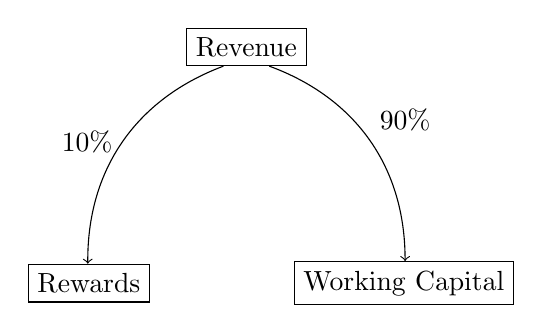
\begin{tikzpicture}
 
 \node[draw] at (-2,-3) (rewards) {Rewards};
 \node[draw] at (2,-3) (workingcapital) {Working Capital};
 \node[draw] at (0,0) (revenue) {Revenue}
    (revenue.-140) edge[bend right=35, ->] node[left]{10{\%}} (rewards)
    (revenue.-40) edge[bend left=35, ->] node[auto]{90{\%}} (workingcapital);
\end{tikzpicture}
\end{center}

\subsection{Claiming Rewards from the reward pot}\label{sec:claimrewards}
Rewards accumulate in the rewards pot. To trigger an actual payout to users (i.e. to make rewards claimable) a special type of proposal is made, proposing that all users should receive a payout based on the reward pot's holdings. 

This reward payout proposal includes the specific currency that should be paid, and only one currency is handled at a time. In the event that the proposal is approved by vote of reputation, then all user's tokens are locked until they claim their payout. Locking is necessary, because the token balance of each account factors into the rewards formula \eqref{eq:reward-claim}. Locking is triggered by incrementing the colony's `most recent payout' counter. 

Our currency contract contains a locking mechanism ensuring that a user cannot move tokens while they have votes to reveal; we use the same mechanism here to ensure that a user cannot move tokens after a payout is approved by the members of the colony but before the user has claimed their rewards. The colony has a counter for each user that is incremented whenever they claim a payout; they can also waive their claim to a payout that will increment this counter.  

While it is of course up to the members of each individual colony to decide, it is advisable that these payout proposals should only be accepted sporadically to keep the gas costs low for the users claiming their payouts, as well as simply to not be a nuisance to the users continually finding their tokens locked.

\textbf{Rewards are only available to accounts that hold both tokens and reputation}, and the amount claimable by each account depends on \emph{both} token balance and reputation (see equation \eqref{eq:reward-claim} below). Therefore we need to have a similar behaviour to `lock' the reputation of the users for the payout. When a payout is activated, the current state of the reputation tree is recorded in the payout itself. Users are paid out according to their reputation in this state, rather than the most recent state, to ensure all users get an appropriate payout and to avoid gaming the system (e.g. ``if I wait until I complete this task, I'll have more reputation and be able to claim more reward'').

\subsubsection*{The Rewards Formula}
The amount that each user ($u_i$) of a colony ($\mathcal{C}$) is entitled to claim ($p_i$) is a function of their colony token holdings ( $t_i$ ) and their total reputation in the colony ($r_i$).

\begin{equation}\label{eq:reward-claim}
 p_i = \left(\frac{t_i r_i}{T \times R}\right)^{\frac{1}{2}} \qquad \textnormal{where} \quad T = \sum\limits_{u_j\in \mathcal{C}} t_j \quad\textnormal{and}\quad R = \sum\limits_{u_j\in \mathcal{C}} r_j
\end{equation}

Note that this is very unlikely to payout all the tokens set aside for a payout - the only way it would do so is if everyone had the same proportion of reputation in the colony as they did proportion of tokens in the colony. However, the geometric average is the natural way to capture influence of two variables, and ensures that large token holders must earn large amounts of reputation to get the most from the payouts. The total tokens issued, total reputation and user reputation in the colony are all provable on-chain at claim time via a merkle proof that the \ascode{ReputationRootHash} (Section \ref{sec:reputationmining}) contains some values claimed by the user; the user's balance of colony tokens is trivial to lookup.

After some sufficiently long period of time (500000 blocks), all unclaimed tokens can be reclaimed by the colony and the payout closed. Any users that have not claimed their payout by that point will still have their tokens locked, and they will remain locked until they issue a transaction waiving their claim to the payout (indeed, they already passively did this by not claiming it in a timely fashion). Unclaimed tokens are returned to the reward pot and become part of the next reward cycle.


\subsubsection{Changing the split}\label{subsec:chaning-the-reward-split}

The 10\%/90\% split between rewards and capital can be altered based on a colony-wide vote of tokens and reputation. It requires a majority of both tokens and reputation in order to pass.




\subsection{The Revenue Model of the Colony Network}\label{sec:networkrevenue}
The Colony Network must be able to sustain itself. In particular, the \rc\ (in control of the colony network and reputation mining) maintains the contracts that underpin the network and develops new functionality for the network, the development of which needs to be paid for. Long term, the development and maintenance of the network (including the reputation system) needs to be financed by the network itself. 

\subsubsection{The Network Fee}\label{sec:networkfee}
We propose a fee that is levied on task payments made. When a user claims payment for a task they have done (Section \ref{sec:claiming-bounty}), some small fraction is paid to the network. 

\begin{center}
 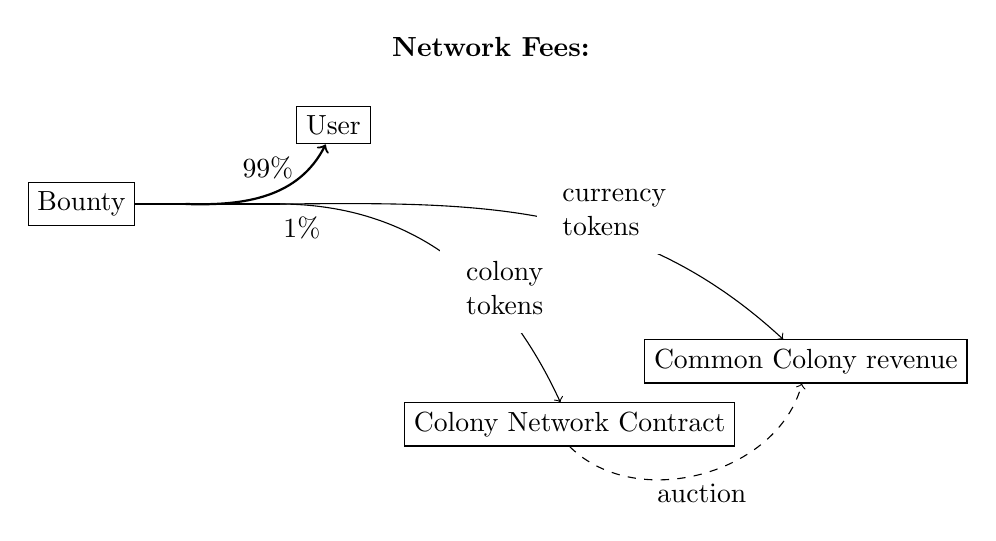
\begin{tikzpicture}
  \node at(0,2) {\textbf{Network Fees:}};
  \node at (-4,0) (dummy) {};
  \node[draw] at (-5.2,0) (bountybox) {Bounty};
  \node at (-2.8,0) (bounty) {}
   (bountybox.east) edge[-, thick] (dummy.east)
   (dummy.east) edge[-] (bounty.east);
   \node at (-2.4,-0.3) {{1\%}};
  \node[draw] at (-2,1) (user) {User};
  \node[draw] at (1,-2.8) (cnc) {Colony Network Contract};
  \node[draw] at (4,-2) (root) {\rc\ revenue}
    (dummy.east) edge[->, bend right=40,out=-25,thick] node[above=2pt] {99{\%}} (user) 
    (dummy.east) edge[->, bend left=30,out=12] node[fill=white,right=10pt] {\begin{tabular}{l} currency \\ tokens\end{tabular}} (root)
    (bounty.east) edge[->, bend left=30,out=35] node[fill=white, below right=-5pt] {\begin{tabular}{l} colony \\ tokens\end{tabular}} (cnc)
    (cnc.south) edge[->, bend right=60, dashed] node[below] {auction} (root)
    ;
 \end{tikzpicture}
\end{center}

The fees thus collected are sent to either the \rc\ (if the payment was in Ether or another whitelisted token) or the Colony Network Contract (if it was in a colony's token).


This idea of a fee is a little unusual for such a decentralised service. One reason why decentralised systems on Ethereum are appealing is that you don't have to pay a fee for the service, other than gas costs. However, we believe that the reputation system will ultimately be appealing enough that a small fee to pay for its existence will be acceptable.

The presence of a fee also means that we have to make some considerations that would be irrelevant to a more traditional decentralised system. For this reason, we will permission the read functions in the \ascode{EternalStorage} contract so that they can only be read by the Colony that owns the \ascode{EternalStorage} contract. This prevents a colony creating a contract that could be used to pay out Ether for tasks without paying the fee based on the status of tasks in the colony.

\subsubsection{The token auction}
The colony tokens collected are auctioned off by the Colony Network Contract, with the auctions denominated in \rcts, the proceeds of which are given to the \rc\ as revenue. These auctions - one for each type of token collected - occur on a regular basis of once a month.

We believe such behaviour would be beneficial for the \rcths\ (whose \rcts\ gain value by having an explicit use) and the \rc\ itself (which turns the fees into \rcts\ which it can then use to fund further development of the network without explicitly buying them back or creating more, diluting existing holders). It also provides an immediate mechanism of price discovery for the colony tokens, which are unlikely to be traded on third-party exchanges until much later in the lifetime of the colony. By auctioning off the collected tokens, we also prevent the \rc\ collecting a large number of different tokens that it has to manage, which would prove cumbersome and annoying for the colony.




\newpage
\section{Special Actions and Example Configurations}\label{sec:special-cases}



% PLAN:

% - move to a separate section the stuff on how a colony manages its own tokens. Include examples in which a token has monetary value and examples in which it doesn't (is used more like an upvote perhaps. This is to set the expectation that not all colony tokens are alike and they are not 'currency' or 'equity' or anything else that you might have thought

% - In this section collect examples such as the salaried position (1 person domain) and reputation bonuses etc and introduce the concept of frontend abstraction.
%
%



\subsection{Proposing an arbitrary transaction by the Colony contract}\label{sec:arbitrary-transaction}
It is desirable to have a mechanism by which a colony can create an arbitrary transaction on the blockchain to interact with contracts and tokens beyond those whitelisted by the network in advance. Such transactions should be rare occurrences with high threshhold requirements.

Formally, proposing that a colony make an arbitrary transaction on the blockchain is no different from an objection; the proposal is to change the value of a special variable from zero to the value of the transaction data of the proposed transaction.\\
Such a proposal requires the entire colony to be able to vote (possibly both token holders and/or reputation holders), as it concerns actions taken `by the contract as a whole'. In the event the proposal is successful, the special variable is set. Another subsequent transaction - able to be made by anyone - is able to call a function that executes the transaction in the special variable, and resets it to zero if successful.

\subsection{Token-weighted, reputation-weighted and hybrid voting}
The majority of decisions in a colony are purely reputation weighted (even though creating a vote requires stake of both tokens and reputation), though there is no reason why a more traditional token-weighted vote shouldn't be available for some decisions, nor a hybrid vote based on both reputation and token holdings. In both of these cases, every account is allowed to vote, and in the case of a hybrid vote, all reputation is eligible to vote. When a hybrid vote takes place, the total reputation and the total token holdings each represent 50\% of the voting weight.

The primary use of a token weighted vote is related to the management of the colony tokens itself; it seems reasonable that the decision and ability to create more tokens should lie with the colony token holders.

 
\subsection{Managing a colony's token supply}\label{sec:colony-token-managements}
\subsubsection{Initial Supply}
When a colony is created, the \ascode{TotalTokenSupply} and the \ascode{TokenIssaunceRate} are set. The former is the total number of colony tokens that will be created and the latter is the rate at which they become available to the colony-wide domain. Just as with any funding proposal (Section \ref{sec:finance}), users can issue a `ping' to update the totals available to the domain.

\subsubsection{Increasing the Token Supply}
In order to increase the \ascode{TotalTokenSupply} and thereby allow for new tokens to be generated, the following events must occur
\begin{itemize}
 \item A proposal is made to increase the value of \ascode{TotalTokenSupply}
 \item The proposal is backed by 10\% of all colony reputation
 \item A colony wide vote of tokens and reputation is held
 \item A majority of reputation voted in favour of the increase
 \item A two-thirds supermajority of tokens voted in favour
 \item Over 30\% of tokens participated in the vote.
\end{itemize}

\subsubsection{Changing the TokenIssaunceRate}
The \ascode{TotalTokenSupply} represents the tokens that the token holders have granted to the reputation holders in order to conduct business: to fund tasks and domains, to hire workers and contributors; especially during the early life of a colony in which it has litte to no revenue in other tokens to fall back on.\\
The \ascode{TokenIssaunceRate} is a measure of how rapidly the colony is able to absorb and allocate the new tokens. If the rate is `too high', tokens will accumulate in the colony wide domain's pot (or other pots lower in the hierarchy); usually this is not a big problem. If the rate is too low however, this signals that the colony has a healthy amount of activity and that the issuance rate has become a bottleneck. In such situations it may be desirable to increase the rate of issuance without necessarily increasing the maximum supply. \\
Increasing and decreasing the \ascode{TokenIssaunceRate} by up to 10\% can be done by the reputation holders alone and this action can be taken no more than once every 4 weeks. Bigger changes to the issuance rate require a double majority of tokens and reputation.

\subsection{Emergency Shutdown}
%
Placeholder\\
How to trigger an emergency shutdown -- the "big red button" we talked about.
Conditions for restarting
%

\subsection{Example Configurations}\label{sec:example-configs}
The Colony Governance Protocol described in this whitepaper is concerned with what happens `on chain', i.e. those actions that directly affect the ethereum blockchain. Users of the network however are not expected to ever interact with the contracts manually; instead they will be using some front-end application that makes all of the network's functionality appear intuitive and simple.\\
In any colony application we expect a certain amount of \textbf{front-end abstraction} in which complex tools and concepts are presented for the users' convenience, and translated in the backgrounnd into a sequence of contract interactions on the colony network.

Front-end abstraction lets us realise certain functionality that doesn't \emph{seem} to be part of our protocol but can actually be coded into the governance system and made usable by a well designed application. Some examples follow.
%

\subsubsection{Salaried Positions}\label{sec:salary}

The work-for-payment model in the colony network is based around tasks, and you'd be forgiven for thinking that this implied colony-worker relationships that are purely transactional. However the system is in fact flexible enough to accomodate a wider range of employment models. One such example is a \emph{salaried position}.

A slaried position could be realised by creating a special domain representing the position to be filled. The domain could be issued the salary through a mandated funding proposal. The hiree would be the only person with reputation within that domain and would be able to withdraw funds by creating and self-assigning placeholder tasks that are funded from the domain's pot. A good frontend could hide these implementation details from the users and render salaried positions differently from regular domains.

\subsubsection{Awarding Reputation Bonuses}

All reputation decays, as described in section \ref{sec:reputation}. This prevents an eternal `reputation aristocracy' and allows reputation to be meaningful even after major changes in the colony token's value. \\
Reputation is awarded when a user receives payment of colony tokens - usually as payout from a task. We can use this mechanim to award users extra reputation provided there is consensus to do so. 

Consider the scenario in which a founder, or an early important contributor to a colony has almost no reputation left by the time the colony starts earning revenue; perhaps the development of the product took a long time or perhaps the reputation decay rate was suboptimally high for the particular colony\footnote{Finding an optimal decay rate for reputation in the network will depend on empirical data collected from early colonies. As with similar constants in this paper, the numerical values may change before the full network is live.}. To get around the limitations of the reputation system and to re-integrate the founder (and make them eligible to receive their just rewards), the colony can create a special `fake' task that is solely designed to award reputation. To qualify for the payout of tokens (and thereby the reputation), the user in question would have to give the same number of tokens back to the colony. Again, a good frontend abstraction could make such reputation awards easy and intuitive.

The important point is that any limitations imposed by the system can be weakened \emph{if there is consensus to do so}. The system should not stand in the way of consensus, it should just provide conflict resolution mechanisms for those times in which there is dissent.


\subsubsection{Objections by non-members}

%
Placeholder\\
explain how without reputation you cannot actually launch an objection, but describe how the frontend can make it easy for the user to propose an objection and ask rep-holders to join. This is analogous to users staking only 10\% of the requirement and waiting for other backers.
%

\subsubsection{Firing members of a colony}

%
Placeholder\\
there isn't really a concept of firing per se, but what we mean here is a special action that sets all of a users reputation to zero.
Threshold, 2/3 of all rep voting in favour, quorum at least 10\%. 
%

Did we want to keep this functionality? I don't remember.


\newpage
\appendix
\newpage
\section{Gas-efficient reputation penalty in dispute resolution}

Once a dispute has been raised and settled one way or the other, the users on the losing side will lose reputation if they have it to lose. If those users lose reputation, some of those on the winning side will therefore gain reputation. If there is a dispute in the reputation mining mechanism, we must be able to calculate on-chain, in a gas-efficient way, whether a specific user was able to lose reputation or not at that time. All of the reputation losses that each user who was involved in the dispute is only represented by a single entry in the `reputation update log`, and so it is necessary to expand upon the process used to do this.

Given that users are able stake small amounts on each objection, an arbitrarily large number of users could theoretically be involved. We must therefore not have any (on-chain) loops in this implementation.

\subsection{Staking}

Let's consider a situation where three users initiate an objection, and two users oppose it with matching funds. In the dispute, the initiating users were found to have been wrong and so will lose their stake.

\begin{table}[h]
\centering
\caption{}
\begin{tabular}{|c|c|c|c|c|c|}
\hline
Stake \# & User  & Staked Amount & $\Sigma^+$ & $\Sigma^-$ \\ \hline
1 & A & 100           & 100                      & 0                                                                       \\ \hline
2 & B & 200           & 300                      & 0                                                                       \\ \hline
3 & C & 300           & 600                      & 0                                                                       \\ \hline
4 & D & -150          & 600                      & -150                                                                    \\ \hline
5 & E & -450          & 600                      & -600                                                                    \\ \hline
\end{tabular}
\end{table}

Let's also assume that all users have the appropriate amount reputation to lose. There are four transfers of reputation that must occur here:

\begin{enumerate}
\item User A loses 100 reputation to User D
\item User B loses 50 reputation to User D
\item User B loses 150 reputation to User E
\item User C loses 300 reputation to User E
\end{enumerate}

Indeed, in a group of $m$ people where some owe the others a debt, the maximum possible of transfers required to make everyone whole is equal to $m-1$. If the reputation being lost has $p$ parents and $c$ children, then there are $2 + 2p + c$ reputation updates that must occur at each of these steps. There are therefore $\left(m-1\right)\times\left(2+2p+c\right)$ reputation updates in total. In the event of a disagreement regarding the reputation state, we must be able to access the $n$th update directly when calculating an update on-chain. This is made possible by additional logging of data when stakes are made.

When a user stakes and opposes some existing stake that does not yet have a counterparty, we record the stakes that it is matching against as well as any remainder.

\begin{table}[ht]
\centering
\caption{}
\begin{tabular}{|c|c|c|c|c|c|}
\hline
Stake & Match From & Match To & Remainder & Tx \# From & Tx \# To\\ \hline
-150  & 1          & 2        & 50      & 1 & 2 \\ \hline
-450  & 2          & 3        & 0       &  3 & 4 \\ \hline
0\tablefootnote{The justification for this line being present is given in section \ref{sec:exactMatching}}  & 0         & 0        & 0 & 5 & 5            \\ \hline
\end{tabular}
\end{table}

When staking, the user supplies the 'Match From' and 'Match To' arguments. These can be checked to be correct on-chain in constant gas by using the values of $\Sigma^+$ and $\Sigma^-$ recorded alongside previous stakes. Then, when a \rcth is asked to prove a particular transaction has been included, they can point to the row in this log that contains that transaction without the contract having to iterate over an arbitrarily long list.

\subsection{Exact matching}\label{sec:exactMatching}

For the `reputation update log' to work correctly, we must know exactly how many reputation updates we have to consider. In the above example, it was $4\times (2+2p+c)$, which could be calculated and recorded easily in the update log. However, consider an example where the staked amounts were

\begin{table}[ht]
\centering
\caption{}
\begin{tabular}{|c|c|c|c|c|c|}
\hline
Stake \# & User  & Staked Amount & $\Sigma^+$ & $\Sigma^-$ \\ \hline
1 & A & 100           & 100                      & 0                                                                       \\ \hline
2 & B & 200           & 300                      & 0                                                                       \\ \hline
3 & C & -100           & 300                      & -100                                                                       \\ \hline
4 & D & -200          & 300                      & -300                                                                    \\ \hline
\end{tabular}
\end{table}

Even though there are four people, only two transfers are required --- from user A to user C, and from user B to user D. This is because the users have accidentally matched themselves exactly, and so one transaction makes two users `whole'. In order to accommodate this possibility in the reputation update log, we insert dummy reputation transfers in the log whenever an exact match occurs:

\begin{table}[ht]
\centering
\caption{}
\begin{tabular}{|c|c|c|c|c|c|}
\hline
Stake & Match From & Match To & Remainder & Tx \# From & Tx \# To \\ \hline
-100  & 1          & 1        & 0   & 1 & 1     \\ \hline
 0 & 0          & 0        & 0      & 2 & 2   \\ \hline
-200 & 2          & 2        & 0    & 3 & 3    \\ \hline
 0 & 0          & 0        & 0      & 4 & 4   \\ \hline
\end{tabular}
\end{table}

These dummy insertions occur whenever the remainder is 0 --- i.e. the stake has matched  the first unmatched stake exactly (or its remainder). This ensures that this log always describes as many transactions as there are people (the last entry is always a dummy transaction as the final transaction will always make two users whole). This means that regardless of how the users have matched up against each other, the event that is recorded in the reputation update log will have a known number of transactions equal to the number of staking users, even if some of those are `null' transactions.

\subsection{Generalisation}

This procedure can also be extended to account for stakes being made in aribtrary orders (i.e. not all of one side followed by all of the other). This can be achieved by making the indices in the `Match From' and `Match To' columns only refer to stakes on one side or the other, and keeping matching lists that map those indices onto the stakes. Altering our first example slightly, we might end up with the stakes in table \ref{appa:modifiedexample} and the log entries in table \ref{appa:modifiedexamplelog}. The list of positive stakes would be [1, 3, 4] and the list of negative stakes would be [2, 5]. The `Match From' and `Match To' indices then refer to the list corresponding to the opposite sign of the stake currently being considered.

\begin{table}[ht]
\centering
\caption{}
\label{appa:modifiedexample}
\begin{tabular}{|c|c|c|c|c|}
\hline
User  & Staked Amount & $\Sigma^+$ & $\Sigma^-$ \\ \hline
A & 100           & 100                      & 0                                                                       \\ \hline
B & -150           & 100                      & -150                                                                     \\ \hline
C & 300           & 400                      & -150                                                                       \\ \hline
D & 200          & 600                      & -150                                                                    \\ \hline
E & -450          & 600                      & -600                                                                    \\ \hline
\end{tabular}
\end{table}

\begin{table}[ht]
\centering
\caption{}
\label{appa:modifiedexamplelog}
\begin{tabular}{|c|c|c|c|c|c|}
\hline
Stake & Match From & Match To & Remainder & Tx \# From & Tx \# To\\ \hline
-150  & 1          & 1        & -50      & 1 & 1 \\ \hline
300   & 1          & 1        & 250      & 2 & 2 \\ \hline
-450  & 2          & 3        & 0       &  3 & 4 \\ \hline
0  & 0         & 0        & 0 & 5 & 5            \\ \hline
\end{tabular}

\end{table}

So for example, in table \ref{appa:modifiedexamplelog}, the stake of -150 is matching against the stake at index 1 in the 'positive stake' list which is stake number 1 i.e. the stake from user A. The stake of 300 is matching against the stake at index 1 in the `negative stake' list, which is stake number 2 i.e. (what remains of) the stake from user B.
\newpage
\clearpage
\section{Reputation Decay Calculation Details}\label{appendix:rep-decay}

Reputation in any skill decays by a factor of two every \repdecayduration\ days. At each update (i.e. after every \miningcycleduration\ hours), the new decayed value ($u_{\rm new}$) is calculated by

$$u_{\rm new} = u_{\rm old} \times \exp\left(-\frac{\ln 2}{\decayfactor}\right) = u_{\rm old} \times \exp\left(-k\right).$$

This calculation is applied separately to each user's skill, as well as the number that represents the total of all of those skills in the colony. Due to rounding error with the integer representation on the blockchain, these numbers will drift away from each other. However, we can show the accumulated error will be negligible. The amount of reputation that will be incorrectly missing after the first iteration will be, on average. $0.5N$ reputation wei, where $N$ is the number of users that have this skill.\footnote{This ignores the incorrectly lost reputation from rounding error introduced when decaying the colony-wide sum of the relevant reputation, but as there is only one total and many more users, ignoring it does not change our conclusions. We also note that there is an implicit assumption here that all users have the same amount of reputation; this is a worst-case assumption, as if it is not true then once some users have lost all their reputation the reputation incorrectly lost on each cycle will drop below $0.5N$.} The 0.5 is the average fractional part lost during each calculation.

After the second iteration, the amount of reputation that is incorrectly missing is

$$0.5N\exp\left(-k\right) + 0.5N.$$


The second term here is the incorrectly lost reputation from this second set of calculations. The factor of $\exp\left(-k\right)$ has been introduced to the term representing the incorrectly lost reputation from the first set of calculations because some of that incorrectly lost reputation would have correctly decayed away by this point, and so it shouldn't be considered incorrectly lost.

It is apparent that this is a geometric series, and after $b$ cycles of reputation update have passed, the amount of reputation incorrectly missing ($R_{\rm m}$) is
$$R_{\rm m} = \frac{N}{2} \left(\frac{1-\exp\left(-bk\right)}{1-\exp\left(-k\right)}\right)$$

\noindent where we have used the standard result for the sum of a geometric series. If we started with $R_0$ reputation, then the ratio of the incorrectly missing reputation to the total the colony believes exists is

$$\frac{R_{\rm m}}{R_0\exp\left(-bk\right)}.$$


This ratio becomes 1 when
$$ b = \frac{1}{k}\ln\left(\frac{2R_{\rm 0}}{N}\left(1-\exp\left(-k\right)\right) +1   \right)$$


\noindent which, for conservative values of $R_0 = 200\times10^{18}$ and $N=1000000$ occurs after 38011 iterations, or over \timetofail\ years for a \miningcycleduration\ hour mining cycle. At this point, even though the colony believes some amount of reputation exists, no users have it, and no users can make decisions related to this type of reputation.

This is the end-of-life for an inactive colony; if no activity takes place in it for \timetofail\ years that is worthy of earning reputation, then the colony will be irrecoverable --- no-one will be able to create tasks to earn further reputation. This seems like a reasonable failure mode for an inactive colony, and it would take longer to reach for smaller colonies (with fewer rounding errors).

We now consider the case of an active colony. If the colony is active and creates $A$ new reputation at every update cycle, how does the ratio between the figure taken to be the total reputation and the incorrectly missing reputation change over time?

$R_{\rm m}$ remains the same in this situation, but the total reputation the colony believes exists increases by $A$ each cycle. After $b$ iterations, we can show that the total reputation the colony believes exists is

$$R_{\rm 0}\exp\left(-bk\right) + A\frac{1-\exp\left(-bk\right)}{1-\exp\left(-k\right)}.$$


As $b$ tends to infinity --- which represents the regime of a colony in a steady state --- the ratio between this and $R_{\rm m}$ tends to
$$\frac{N}{2A}$$

\noindent i.e. for the discrepancy to be small between what the colony thinks the total reputation inside it is and the sum of all users' reputations, the reputation earned in each cycle should, on average, be much larger than the number of users. Given that reputation will be expressed in terms of numbers on the order of $10^{18}$, this seems assured.

For calculating the exponential decay, we will use the first-order Taylor expansion of the exponential decay i.e. we approximate $\exp\left(-k\right)$ as $1-k$. Given that $k$ is small, this will be a good approximation --- the second order term is on the order of $10^{-7}$. This error will cause all reputations to decay slightly faster than an exponential, but otherwise will have no effect.

When calculating the decay, in order to accommodate the fact that we are multiplying by a value close to one and only integers are available in Solidity, we will multiply the user's reputation by $K(1-k)$ (calculated off-chain), for some large value of $K$, and then divide by the same large factor $K$.



% {Bibliography}
\begin{thebibliography}{9}
  
  
\bibitem{TruebitWhitepaper}
  Jason Teutsch \& Christian Reitwießner,
  \emph{A scalable verification solution for blockchains}
  \verb| people.cs.uchicago.edu/~teutsch/papers/truebit.pdf |
  
\bibitem{ColonyVoting}
  Elena Dimitrova,
  \emph{Token-weighted voting implementation}
  \verb| blog.colony.io/token-weighted-voting-implementation-part-1-72f836b5423b |
  
\bibitem{KeynesianBeauty}
  economicsnetwork.ac.uk,
  \emph{References for Keynesian Beauty Contest}
  \verb| www.economicsnetwork.ac.uk/sites/default/files/Ashley/6%20References%20for%20KBC.pdf |

\bibitem{MerkleTrees}
  Georg Becker,
  \emph{Merkle Signature Schemes, Merkle Trees and Their Cryptanalysis}
  \verb| www.emsec.rub.de/media/crypto/attachments/files/2011/04/becker_1.pdf |

\bibitem{MerkleInEthereum}
  Vitalik Buterin,
  \emph{Merkling in Ethereum}
  \verb| blog.ethereum.org/2015/11/15/merkling-in-ethereum/ |
  
\bibitem{YellowPaper}
  Gavin Wood et el.
  The Ethereum ``Yellow Paper''
  \emph{A secure decentralised generalised transaction ledger}
  \verb| ethereum.github.io/yellowpaper/paper.pdf |
  
\bibitem{UpgradingContracts}
  Elena Dimitrova,
  \emph{Writing upgradable contracts in Solidity}
  \verb| blog.colony.io/writing-upgradeable-contracts-in-solidity-6743f0eecc88 |
  
\bibitem{erc20}
  Fabian Vogelsteller et al.
  \emph{ERC: Token standard \#20}
  \verb| github.com/ethereum/EIPs/issues/20 |
  
\end{thebibliography}

\end{document}
